


% ============================================================
%  Stellen_presentation.tex  —  CORRECTED VERSION
%  Fixes applied:
%   1. Removed \begingroup / \setslidetemplate / \endgroup blocks
%   2. Removed \sechead and \refcite (Auriga-only commands)
%   3. Fixed equation* with &=& → align*
%   4. Fixed \multirow{Metric} → \multirow{2}{*}{Metric}
%   5. Removed duplicate \end{frame}
%   6. Colors mainblue / accentblue must be defined in preamble
%   7. \usepackage{multirow} must be in preamble
% ============================================================

% ── TITLE FRAME ─────────────────────────────────────────────
{
  \setbeamercolor{page number in head/foot}{fg=background canvas.bg}
  \begin{frame}
    \begin{tikzpicture}[remember picture, overlay]
      \node[anchor=north west, xshift=1em, yshift=-1em] at (current page.north west) {
        
\includegraphics[width=3cm]{logo.png}
      };
    \end{tikzpicture}

    \titlepage

    \begin{center}
      \qrcode[height=2.8cm]{https://github.com/Xaleed/DirichletRF.git}
      \vspace{0.1cm}
      {\small GitHub repository}
    \end{center}
  \end{frame}
}


% ── OVERVIEW ────────────────────────────────────────────────
\begin{frame}{What is This Talk About?}

\vspace{2em}
\vspace{1.5em}

\begin{itemize}
  \item[\textcolor{blue}{\large$\blacktriangleright$}] \textbf{Compositional Data} -- Fundamental properties and modeling challenges
  \vspace{1em}

  \item[\textcolor{blue}{\large$\blacktriangleright$}] \textbf{Literature Review} -- Historical development and ongoing debates
  \vspace{1em}

  \item[\textcolor{blue}{\large$\blacktriangleright$}] \textbf{Machine Learning with Random Forests} -- Capturing complex relationships
  \vspace{1em}

  \item[\textcolor{blue}{\large$\blacktriangleright$}] \textbf{Comparative Results} -- Assessing predictive performance
  \vspace{1em}

  \item[\textcolor{blue}{\large$\blacktriangleright$}] \textbf{DirichletRF R Package} -- Implementation and practical use
\end{itemize}

\vspace{2em}
\end{frame}


% ── COMPOSITIONAL DATA ──────────────────────────────────────
\begin{frame}{Compositional data}

\only<1>{
  \vspace{1em}

  A simplex is a convex space of all vectors with non-negative components that sum to a constant.

  \begin{center}
  \colorbox{blue!10}{\parbox{0.8\textwidth}{
  \begin{center}
  \[
    S^c_k = \left\{ (y_1, \dots, y_k)^\top \in \mathbb{R}^k \,\middle|\, y_i \geq 0,\ \sum_{i=1}^k y_i = \textcolor{blue}{c} \right\}
  \]
  \end{center}
  }}
  \end{center}

  It is common to set \(\textcolor{blue}{c = 1}\). We refer to data from this space as \emph{compositional data}.
}

\only<2>{
  \textbf{A practical view of compositional data}

  \vspace{0.3cm}
  Let $\mathbf{Y} = (Y_1, Y_2, \dots, Y_K)$ be a vector with positive components.

  \vspace{0.3cm}
  The compositional transformation is defined as:
  \[
    \mathbf{S} = \left( \frac{Y_1}{\sum_{i=1}^K Y_i}, \dots, \frac{Y_K}{\sum_{i=1}^K Y_i} \right)
  \]

  \vspace{0.3cm}
  This vector lies in the simplex space.

  \vspace{0.5cm}
  However, in this transformation we lose information about the \textbf{absolute scale}, and we cannot uniquely recover the original vector.

  But we preserve the \textbf{relative information}. In particular, for any two components $i$ and $j$:
  \[
    \frac{Y_i}{Y_j} = \frac{S_i}{S_j}
  \]
}

\only<3>{
  Consider a job application pool of $50$ applicants classified by academic background.
  \vspace{0.3cm}

  \begin{columns}
    \begin{column}{0.4\textwidth}
      \[ \mathbf{Y} = (10, 15, 25) \]
    \end{column}
    \begin{column}{0.5\textwidth}
      \begin{tabular}{lr}
        Mathematics      & 10 \\
        Statistics       & 15 \\
        Computer Science & 25 \\
      \end{tabular}
    \end{column}
  \end{columns}

  \vspace{0.3cm}
  We normalize this vector to obtain a compositional representation:
  \vspace{0.2cm}

  \begin{columns}
    \begin{column}{0.5\textwidth}
      \[ \mathbf{s}(\mathbf{Y}) = \left(\frac{10}{50}, \frac{15}{50}, \frac{25}{50}\right) \]
    \end{column}
    \begin{column}{0.4\textwidth}
      \[ = (0.2, 0.3, 0.5) \]
      Interpreted as proportions.
    \end{column}
  \end{columns}

  \vspace{0.2cm}
  Multiplying by $100$ gives percentages:
  \vspace{0.2cm}

  \begin{columns}
    \begin{column}{0.5\textwidth}
      \[ 100 \cdot \mathbf{s}(\mathbf{Y}) = (20\%, 30\%, 50\%) \]
    \end{column}
    \begin{column}{0.4\textwidth}
      \textbf{Key idea:} The information is identical --- only the scale changes.
    \end{column}
  \end{columns}
}

\end{frame}


% ── CORRELATION ─────────────────────────────────────────────
\begin{frame}{Correlation}

\only<1>{
  \begin{columns}
    \column{0.5\textwidth}
    \textbf{Original Data (Counts)}
    \vspace{0.2cm}
    \begin{center}
    \begin{tabular}{lccc}
      \hline
       & Math & Stats & CS \\
      \hline
      Job 1 & 48  & 230 & 59  \\
      Job 2 & 286 & 181 & 73  \\
      Job 3 & 286 & 98  & 147 \\
      Job 4 & 35  & 14  & 12  \\
      Job 5 & 255 & 104 & 235 \\
      $\vdots$ & $\vdots$ & $\vdots$ & $\vdots$ \\
      \hline
    \end{tabular}
    \end{center}
    \vspace{0.2cm}
    \[ \mathrm{corr}(\text{Math},\,\text{Stats}) = 0.087 \]
    \column{0.5\textwidth}
  \end{columns}
}

\only<2>{
  \begin{columns}
    \column{0.5\textwidth}
    \textbf{Original Data (Counts)}
    \vspace{0.2cm}
    \begin{center}
    \begin{tabular}{lccc}
      \hline
       & Math & Stats & CS \\
      \hline
      Job 1 & 48  & 230 & 59  \\
      Job 2 & 286 & 181 & 73  \\
      Job 3 & 286 & 98  & 147 \\
      Job 4 & 35  & 14  & 12  \\
      Job 5 & 255 & 104 & 235 \\
      $\vdots$ & $\vdots$ & $\vdots$ & $\vdots$ \\
      \hline
    \end{tabular}
    \end{center}
    \vspace{0.2cm}
    \[ \mathrm{corr}(\text{Math},\,\text{Stats}) = 0.087 \]
    \column{0.5\textwidth}
    \textbf{Compositional Data (Normalized to 100)}
    \vspace{0.2cm}
    \begin{center}
    \begin{tabular}{lccc}
      \hline
       & Math & Stats & CS \\
      \hline
      Job 1 & 14.2 & 68.2 & 17.5 \\
      Job 2 & 53.0 & 33.5 & 13.5 \\
      Job 3 & 53.9 & 18.5 & 27.7 \\
      Job 4 & 57.4 & 23.0 & 19.7 \\
      Job 5 & 42.9 & 17.5 & 39.6 \\
      $\vdots$ & $\vdots$ & $\vdots$ & $\vdots$ \\
      \hline
    \end{tabular}
    \end{center}
    \vspace{0.2cm}
    \[ \mathrm{corr}(X_{\text{math}},\, X_{\text{stats}}) = -0.874 \]
  \end{columns}
  \vspace{0.1cm}
  What does $\mathrm{corr}(X_{\text{math}},\, X_{\text{stats}}) = -0.874$ mean?
  \vspace{0.1cm}
  \begin{alertblock}{Warning}
    A common mistake is to interpret this correlation as if it were computed on the raw counts.
  \end{alertblock}
}

\only<3>{
  \begin{columns}
    \column{0.5\textwidth}
    \textbf{Original Data (Counts)}
    \vspace{0.2cm}
    \begin{center}
    \begin{tabular}{lccc}
      \hline
       & Math & Stats & CS \\
      \hline
      Job 1 & ? & ? & ? \\
      Job 2 & ? & ? & ? \\
      Job 3 & ? & ? & ? \\
      Job 4 & ? & ? & ? \\
      Job 5 & ? & ? & ? \\
      $\vdots$ & $\vdots$ & $\vdots$ & $\vdots$ \\
      \hline
    \end{tabular}
    \end{center}
    \vspace{0.2cm}
    \[ \mathrm{corr}(\text{Math},\,\text{Stats}) = \text{?} \]
    \column{0.5\textwidth}
    \textbf{Compositional Data (Normalized to 100)}
    \vspace{0.2cm}
    \begin{center}
    \begin{tabular}{lccc}
      \hline
       & Math & Stats & CS \\
      \hline
      Job 1 & 14.2 & 68.2 & 17.5 \\
      Job 2 & 53.0 & 33.5 & 13.5 \\
      Job 3 & 53.9 & 18.5 & 27.7 \\
      Job 4 & 57.4 & 23.0 & 19.7 \\
      Job 5 & 42.9 & 17.5 & 39.6 \\
      $\vdots$ & $\vdots$ & $\vdots$ & $\vdots$ \\
      \hline
    \end{tabular}
    \end{center}
    \vspace{0.2cm}
    \[ \mathrm{corr}(X_{\text{math}},\, X_{\text{stats}}) = -0.874 \]
  \end{columns}
  \vspace{0.1cm}
  \begin{alertblock}{Warning}
    In cases where only compositional data are observed, the original dependence structure is unknown and cannot be uniquely recovered from the simplex representation.
  \end{alertblock}
}

\end{frame}


% ── SPURIOUS CORRELATION ────────────────────────────────────
\begin{frame}{Spurious Correlation}

\only<1>{
  \begin{block}{Pearson (1897)}
    Ratios that share a common denominator are correlated even when the original variables are \emph{completely independent}.
  \end{block}

  \vspace{0.4em}

  \begin{columns}[t]
    \begin{column}{0.38\textwidth}
      \textbf{Original vector:}\\[4pt]
      $\mathbf{Y} = (Y_1, Y_2, \ldots, Y_K) \in \mathbb{R}_+^K$
    \end{column}
    \begin{column}{0.58\textwidth}
      \textbf{Simplex (normalized):}\\[4pt]
      $\mathbf{s}(\mathbf{Y}) = \!\left(\dfrac{Y_1}{S},\, \dfrac{Y_2}{S},\, \ldots,\, \dfrac{Y_K}{S}\right), \quad S = \sum_{j=1}^{K} Y_j$
    \end{column}
  \end{columns}

  \vspace{0.5em}
  \rule{\textwidth}{0.3pt}
  \vspace{0.3em}

  Even if $\operatorname{corr}(Y_1,\, Y_2) = 0$, we usually observe:
  \[
    \boxed{\operatorname{corr}\!\left(\frac{Y_1}{S},\,\frac{Y_2}{S}\right) \neq 0}
  \]
}

\end{frame}


% ── STATISTICAL DIFFICULTIES ────────────────────────────────
\begin{frame}{Statistical Difficulties}

\only<1>{
  \vspace{0.4em}
  \[
  \Sigma_{\mathbf{X}} =
  \begin{pmatrix}
    \operatorname{Var}(X_1)     & \operatorname{cov}(X_1,X_2) & \cdots & \operatorname{cov}(X_1,X_K) \\
    \operatorname{cov}(X_2,X_1) & \operatorname{Var}(X_2)     & \cdots & \operatorname{cov}(X_2,X_K) \\
    \vdots                      & \vdots                       & \ddots & \vdots \\
    \operatorname{cov}(X_K,X_1) & \operatorname{cov}(X_K,X_2) & \cdots & \operatorname{Var}(X_K)
  \end{pmatrix}
  \in \mathbb{R}^{K \times K}
  \]
  \vspace{0.2em}
  The \textbf{last row (and column) is linearly determined} by the others via the sum-to-constant constraint, confirming $\operatorname{rank}(\Sigma_{\mathbf{X}}) = K-1$.
}

\only<2>{
  The sum-to-constant constraint causes the \textbf{sample covariance matrix to be singular}:
  \[
    \sum_{i=1}^{K} \operatorname{cov}(X_1, X_i)
    = \operatorname{cov}\!\left(X_1,\, \sum_{i=1}^K X_i\right)
    = \operatorname{cov}(X_1,\, 1) = 0
  \]
  \[
    \Rightarrow\quad \sum_{i=2}^{K} \operatorname{cov}(X_1, X_i) = -\operatorname{Var}(X_1).
  \]

  \vspace{0.3em}
  $\Sigma_{\mathbf{X}}$ has rank $K-1$ $\;\Rightarrow\;$ \textbf{not invertible}.

  \vspace{0.5em}
  \begin{columns}[T]
    \begin{column}{0.48\textwidth}
      \textbf{Technical consequence:}
      \begin{itemize}
        \item Regression, LDA, and standard PCA all require $\Sigma^{-1}$ -- unavailable.
      \end{itemize}
    \end{column}
    \begin{column}{0.48\textwidth}
      \textbf{Conceptual consequence:}
      \begin{itemize}
        \item No universally accepted definition of correlation for compositional data exists yet.
      \end{itemize}
    \end{column}
  \end{columns}
}

\end{frame}


% ── LOG-RATIO SECTION TITLE ─────────────────────────────────
\begin{frame}{Log-Ratio Transformations}
  \centering
  \vfill
  \textbf{\Large Log-Ratio Transformations}
  \vfill
\end{frame}


% ── ALR ─────────────────────────────────────────────────────
\begin{frame}[t]{Additive Log-Ratio (ALR) Transformation}

  \vspace{0.2cm}

  \textbf{Definition.}
  For $\mathbf{x}=(x_1,\ldots,x_K)^\top \in \mathcal{S}^{K-1}$, choose a reference component $x_K$:

  \vspace{0.35cm}
  \[
    \mathrm{ALR}(\mathbf{x})
    = \left( \log\frac{x_1}{x_K},\; \log\frac{x_2}{x_K},\;\ldots,\; \log\frac{x_{K-1}}{x_K} \right)
    \in \mathbb{R}^{K-1}
  \]

  \vspace{0.3cm}

  \only<1>{
    \begin{itemize}\setlength\itemsep{6pt}
      \item Maps compositional data to Euclidean space $\mathbb{R}^{K-1}$
      \item Covariance matrix becomes full rank $\Rightarrow$ standard methods applicable
      \item \textcolor{red!70!black}{Depends on choice of reference component $x_K$}
    \end{itemize}

    \vspace{0.3cm}
    Aitchison (1982)
  }

\end{frame}


% ── CLR ─────────────────────────────────────────────────────
\begin{frame}[t]{Centered Log-Ratio (CLR) Transformation}

  \vspace{0.2cm}

  \textbf{Definition.} Normalize by the geometric mean:

  \vspace{0.3cm}
  \[
    \mathrm{CLR}(\mathbf{x})
    = \left( \log\frac{x_1}{g(\mathbf{x})},\ldots, \log\frac{x_K}{g(\mathbf{x})} \right)
    \in \mathbb{R}^K
  \]
  \[
    g(\mathbf{x}) = \left(\prod_{j=1}^K x_j\right)^{1/K}
  \]

  \vspace{0.2cm}

  \only<1>{
    \begin{itemize}\setlength\itemsep{6pt}
      \item Symmetric representation (no reference component)
      \item Components satisfy: $\sum_{i=1}^K \mathrm{CLR}_i = 0$
      \item Still lies in a constrained subspace $\Rightarrow$ singular covariance
    \end{itemize}

    \vspace{0.3cm}
    Aitchison (1982)
  }

\end{frame}


% ── ILR ─────────────────────────────────────────────────────
\begin{frame}[t]{Isometric Log-Ratio (ILR) Transformation}

  \vspace{0.2cm}

  \textbf{Definition.} (Barcel\'{o}-Vidal et al.\ (2001); Egozcue et al.\ (2003))

  By projecting the CLR coordinates onto an orthonormal basis, usually with a $(K{-}1)\!\times\! K$ Helmert sub-matrix $\mathbf{H}$, we obtain the isometric log-ratio transformation, or ILR:

  \vspace{0.2cm}
  \[
    \mathrm{ILR}(\mathbf{x})
    = \mathbf{H}\;\mathrm{CLR}(\mathbf{x})
    = (z_1,\;z_2,\;\ldots,\;z_{K-1})
    \in\mathbb{R}^{K-1}
  \]
  \[
    \mathbf{H}\mathbf{H}^\top = \mathbf{I}_{K-1} \quad\text{(rows orthonormal)}
  \]

  \only<1>{
    \begin{alertblock}{Properties.}
      \begin{itemize}\setlength\itemsep{4pt}
        \item Resolves CLR singularity: $\Sigma_{\mathrm{ILR}}$ is \textbf{full rank}
        \item Any $(K{-}1)\!\times\!K$ orthonormal matrix works in place of $\mathbf{H}$
        \item \textcolor[HTML]{2A9D8F}{\textbf{Isometric:}} Distances preserved by $\mathbf{H}$:
          $\|\mathrm{CLR}(\mathbf{x})-\mathrm{CLR}(\mathbf{y})\| = \|\mathrm{ILR}(\mathbf{x})-\mathrm{ILR}(\mathbf{y})\|$
      \end{itemize}
    \end{alertblock}
  }

\end{frame}


% ── ONE IDEA: TRANSFORMING (table 1) ────────────────────────
\begin{frame}{One Idea: Transforming to Real Space}

\only<1>{
  \begin{itemize}
    \item[1)] CoDA School: Some researchers claim that log-ratio transformations are necessary for compositional data.
    \item[2)] To support this view, a set of principles (CoDA principles) was proposed that any valid compositional method should satisfy.
  \end{itemize}

  \vspace{0.2cm}
  \renewcommand{\arraystretch}{1.35}
  \setlength{\tabcolsep}{8pt}

  \begin{tabular}{>{\bfseries}l l >{\footnotesize\itshape\color{gray}}l}
    \toprule
    \rowcolor{mainblue}
    \color{white}Method & \color{white}Formula & \color{white}Reference \\
    \midrule
    \rowcolor{accentblue!20}
    ALR & $\log x_i - \log x_K$ & Aitchison (1982) \\
    \rowcolor{accentblue!20}
    CLR & $\log x_i - K^{-1}\sum_{j=1}^{K} \log y_j$ & Aitchison (1983) \\
    \rowcolor{accentblue!20}
    ILR & $\mathbf{H}\!\left(\log y_i - K^{-1}\sum_{j=1}^{K} \log y_j\right)$ & Egozcue et al.\ (2003) \\
    \midrule
    \bottomrule
  \end{tabular}
}

\only<2>{
  \begin{alertblock}{Principles of CODA}
    \begin{itemize}
      \item \textbf{scale invariance},
      \item \textbf{permutation invariance}, and
      \item \textbf{subcompositional coherence}: If $\Delta_p(\mathbf{x}, \mathbf{y})$ denotes a distance measure between compositions with $p$ parts, then
        \[
          \Delta_k(\mathbf{x}, \mathbf{y}) \geq \Delta_d(\mathbf{x}_d, \mathbf{y}_d),
        \]
        where $\mathbf{x}, \mathbf{y}$ are compositions with $k$ parts, and $\mathbf{x}_d, \mathbf{y}_d$ are corresponding subcompositions with $d < k$ parts.
    \end{itemize}
  \end{alertblock}

  \begin{itemize}
    \item[1)] \textbf{Basic mathematical operations} on the simplex (perturbation, powering, inner product)
    \item[2)] \textbf{Measures of central tendency}: simplicial means and medians
    \item[3)] \textbf{Distances and metrics} between compositions
    \item[4)] \textbf{Distributions} defined on or adapted to the simplex
  \end{itemize}
}

\end{frame}


% ── DEBATES ─────────────────────────────────────────────────
\begin{frame}{Debates}
\begin{itemize}
  \item[\textcolor{blue}{\large$\blacktriangleright$}] These transformations were introduced by Aitchison in 1982, but the principles of CoDA have been developing over the years since then.
  \item[\textcolor{blue}{\large$\blacktriangleright$}] In 1989, Watson and Philip challenged both the log-ratio approach and the notion that these principles should be treated as universal requirements, proposing alternatives such as directional approaches.
  \item[\textcolor{blue}{\large$\blacktriangleright$}] They exchanged ideas for three years, and \textit{Mathematical Geology} published their letters in response to each other.
  \item[\textcolor{blue}{\large$\blacktriangleright$}] What began as a methodological disagreement gradually escalated in tone, becoming increasingly confrontational.
  \item[\textcolor{blue}{\large$\blacktriangleright$}] The debate ultimately ended with Watson's withdrawal --- Aitchison's use of the word \textcolor{red}{``stupid''} to dismiss Watson's contributions led Watson to disengage from further discussion.
\end{itemize}
\end{frame}

\begin{frame}{Debates}
\begin{itemize}
  \item[1.] Following this period, the CoDA framework grew increasingly dominant:
  \begin{itemize}
    \item[1.1] Aitchison continued to advance the framework through numerous publications, including an influential book.
    \item[1.2] A broader research community developed around the field that supported these principles.
  \end{itemize}
  \item[2.] As a result, alternative approaches received considerably less attention.
\end{itemize}
\end{frame}

\begin{frame}{Debates}
\only<1>{
  The CoDA school has redefined these principles several times in response to criticism.

  \begin{alertblock}{Zier \& Rehder (1998, 2001)}
    They pointed out that even Aitchison's own earlier work did not strictly satisfy the later CoDA definition of scale invariance.
  \end{alertblock}

  \begin{alertblock}{Scealy \& Welsh (2014)}
    The CoDa Principles act as a \textbf{gatekeeping criterion}: valid and useful methods have been dismissed simply for not conforming to them.

    \vspace{0.2cm}
    This is \textbf{unusual, perhaps unique, in statistical data analysis}.
  \end{alertblock}
}
\end{frame>


% ── ONE IDEA: TRANSFORMING (full table) ─────────────────────
\begin{frame}{One Idea: Transforming to Real Space}

\only<1>{
  \framesubtitle{A transformation $\mathcal{S}^{K-1} \to \mathbb{R}^{K-1}$ unlocks standard inference: regression, PCA, LDA}

  \vspace{0.2cm}
  \renewcommand{\arraystretch}{1.35}
  \setlength{\tabcolsep}{8pt}

  \begin{tabular}{>{\bfseries}l l >{\footnotesize\itshape\color{gray}}l}
    \toprule
    \rowcolor{mainblue}
    \color{white}Method & \color{white}Formula & \color{white}Reference \\
    \midrule
    \rowcolor{accentblue!20}
    ALR & $\log y_i - \log y_K$ & Aitchison (1982) \\
    \rowcolor{accentblue!20}
    CLR & $\log y_i - K^{-1}\sum_{j=1}^{K} \log y_j$ & Aitchison (1983) \\
    \rowcolor{accentblue!20}
    ILR & $\mathbf{H}\!\left(\log y_i - K^{-1}\sum_{j=1}^{K} \log y_j\right)$ & Egozcue et al.\ (2003) \\
    \midrule
    {\normalfont $\alpha$}            & {\footnotesize $\mathbf{H}[K_\alpha^{-1}(\mathbf{y} \otimes \alpha)]$}                              & Tsagris et al.\ (2011) \\
    {\normalfont BC$_1$}              & {\footnotesize $\lambda^{-1}\!\left[(y_i / y_K)^\lambda - 1\right]$}                               & Aitchison (2003) \\
    {\normalfont BC$_2$}              & {\footnotesize $\theta^{-1}(y_i^\theta - 1)$}                                                      & Greenacre (2010) \\
    {\normalfont Hyper-spherical}     & {\footnotesize $\arccos\!\left(\dfrac{y_i}{\prod_{j=i+1}^{K} y_j}\right)$}                         & Wang et al.\ (2007) \\
    {\normalfont Square root}         & {\footnotesize $\sqrt{y_i}$}                                                                       & Stephens (1982) \\
    \bottomrule
  \end{tabular}

  \vspace{0.2cm}
  {\small\textbf{Key:} ALR, CLR, ILR are the most widely used; all resolve singularity of $\Sigma_{\mathbf{X}}$ by mapping to unconstrained $\mathbb{R}^{K-1}$.}
}

\end{frame}


% ── ML SECTION TITLE ────────────────────────────────────────
\begin{frame}{Machine learning for CoDA}
  \centering
  \vfill
  \textbf{\Large Machine learning for CoDA}
  \vfill
\end{frame}


% ── ML: RANDOM FOREST ───────────────────────────────────────
\begin{frame}{Machine learning: Random Forest}

\begin{itemize}
  \item \textbf{Why machine learning?}
    For responses that are compositional: many predictors with complex non-linear patterns that traditional models cannot capture.

  \item \textbf{Common approaches}:
    Apply ML models without considering the simplex geometry, or transform data (with log-ratio transformations) to real space (risking distortion and bias).

  \item \textbf{Why Random Forests?}
    RFs are flexible and their splitting rules can be easily adapted to respect the simplex structure.

  \item PhD of van der Westhuizen (2024) inspired the idea to use tree splitting to account for CoDA.
\end{itemize}

\end{frame}


% ── ML FRAMEWORK ────────────────────────────────────────────
\begin{frame}{Machine learning framework}

\begin{itemize}
  \item[\textcolor{blue}{\large$\blacktriangleright$}] Given a sample size $n$ and $m$ covariates:
    \[
      \mathbf{X} \in \mathbb{R}^{n \times m} \quad \text{(covariate matrix)}, \qquad
      \mathbf{Y} \in \mathbb{R}^{n \times k} \quad \text{(response matrix)}
    \]

  \item[\textcolor{blue}{\large$\blacktriangleright$}] Each row of $\mathbf{Y}$ is a compositional vector:
    \[
      Y_{i,j} > 0 \quad \text{for all } i, j, \qquad \sum_{j=1}^k Y_{i,j} = 1
    \]

  \item[\textcolor{blue}{\large$\blacktriangleright$}] Goal: learn a mapping
    \[ \mathbf{x} \;\longrightarrow\; \mathbf{y} \]
    respecting the simplex geometry
    \vspace{0.8em}

  \item[\textcolor{blue}{\large$\blacktriangleright$}] After training:
    \begin{itemize}
      \item Predict compositional responses for new inputs
      \item Estimate conditional distribution of responses
    \end{itemize}
\end{itemize}

\end{frame}


% ── RANDOM FOREST: TREE ─────────────────────────────────────
\begin{frame}{Random forest: tree}
\centering
\only<1>{
  \begin{columns}
    \begin{column}{0.4\linewidth}
      \begin{figure}[h]
      \centering
      \begin{tikzpicture}[
        node distance=0.8cm,
        box/.style={rectangle, draw, minimum width=1.8cm, minimum height=0.8cm, text centered, font=\small},
        dot/.style={circle, fill=black, minimum size=2pt, inner sep=0pt},
        arrow/.style={->, thick}
      ]
        \node[box] (parent) {$S$=\\$(y_1, y_2, ..., y_n)$};
        \node[dot, below=0.6cm of parent] (split) {};
        \node[box, below left=0.8cm and 1.2cm of split] (left) {$S_1$};
        \node[box, below right=0.8cm and 1.2cm of split] (right) {$S_2$};
        \draw (parent) -- (split);
        \draw (split) -- (left);
        \draw (split) -- (right);
        \node[right=1.5cm of split, font=\small] (loss) {$\texttt{criteria} = $ ?};
        \draw[arrow] (split) -- (loss);
      \end{tikzpicture}
      \end{figure}
    \end{column}

    \begin{column}{0.6\linewidth}
      \vspace{1cm}
      $\qquad \qquad$A binary decision tree

      \resizebox{1\linewidth}{!}{%
      \begin{tikzpicture}[
        level/.style={sibling distance=60mm/#1},
        every node/.style={circle, draw, minimum size=8mm, font=\tiny},
        dots/.style={draw=none, font=\large}
      ]
      \node {Root}
        child {
          node {L1}
          child { node {L2} child { node[dots] {$\vdots$} } child { node[dots] {$\vdots$} } }
          child { node {L2} child { node[dots] {$\vdots$} } child { node[dots] {$\vdots$} } }
        }
        child {
          node {R1}
          child { node {L2} child { node[dots] {$\vdots$} } child { node[dots] {$\vdots$} } }
          child { node {L2} child { node[dots] {$\vdots$} } child { node[dots] {$\vdots$} } }
        };
      \end{tikzpicture}}
    \end{column}
  \end{columns}
}
\end{frame}


% ── MSE SPLITTING (diagram + formula) ───────────────────────
\begin{frame}{}

\only<1>{
  \frametitle{MSE splitting}

  \begin{tikzpicture}[
    node distance=1cm and 1cm,
    every node/.style={font=\small},
    data/.style={rectangle, draw, align=center, fill=blue!5, rounded corners, inner sep=5pt},
    split/.style={->, thick},
    highlight/.style={->, red, thick, dashed}
  ]
    \node[data] (parent) {
      \textbf{Parent Node} \\[0.15cm] Covariate: $X^{n \times m}$ \\ Response: $Y^{n \times k}$
    };
    \node[data, below left=of parent] (left) {
      \textbf{Left Child} \\[0.1cm] Covariate: $X^{n_1 \times m}$ \\ Response: $Y^{n_1 \times k}$ \\[0.1cm]
      MSE $= \text{MSE}(Y^{n_1 \times k},c,i)$
    };
    \node[data, below right=of parent] (right) {
      \textbf{Right Child} \\[0.1cm] Covariate: $X^{n_2 \times m}$ \\ Response: $Y^{n_2 \times k}$ \\[0.1cm]
      MSE $= \text{MSE}(Y^{n_2 \times k},c,i)$
    };
    \draw[split] (parent) -- node[midway, left] (leftlabel) {$x_{ij} \leq c$} (left);
    \draw[split] (parent) -- node[midway, right] (rightlabel) {$x_{ij} > c$} (right);
    \node[red, left] (opt_i) at ([xshift=-1.5cm, yshift=1.2cm]leftlabel) {$(c,i)=?$};
    \node[red, right] (opt_c) at ([xshift=1.5cm, yshift=1.2cm]rightlabel) {$(c,i)=?$};
    \draw[highlight] (opt_i) -- (leftlabel.west);
    \draw[highlight] (opt_c) -- (rightlabel.east);
  \end{tikzpicture}

  % FIX: was equation* with &=& which is illegal; use align*
  \begin{align*}
    (c^*, i^*)
    &= \operatorname{argmin}_{i,c} \left( \text{MSE}(Y^{n_1 \times k},c,i) + \text{MSE}(Y^{n_2 \times k},c,i) \right) \\
    &= \arg\min_{c,j}
      \left\{
        \frac{n_1(c,j)}{n} \sum_{m=1}^k \sum_{i=1}^{n_1(c,j)} (y_{im}-\bar{y}_{m}^{n_1(c,j)})^2
        +
        \frac{n_2(c,j)}{n} \sum_{m=1}^k \sum_{i=1}^{n_2(c,j)} (y_{im}-\bar{y}_{m}^{n_2(c,j)})^2
      \right\}.
  \end{align*}
}

\only<2>{
  \frametitle{MSE splitting}

  \begin{tikzpicture}[
    node distance=1cm and 1cm,
    every node/.style={font=\small},
    data/.style={rectangle, draw, align=center, fill=blue!5, rounded corners, inner sep=5pt},
    split/.style={->, thick},
    highlight/.style={->, red, thick, dashed}
  ]
    \node[data] (parent) {
      \textbf{Parent Node} \\[0.15cm] Covariate: $X^{n \times m}$ \\ Response: $Y^{n \times k}$
    };
    \node[data, below left=of parent] (left) {
      \textbf{Left Child} \\[0.1cm] Covariate: $X^{n_1 \times m}$ \\ Response: $Y^{n_1 \times k}$ \\[0.1cm]
      MSE $= \text{MSE}(Y^{n_1 \times k},c,i)$
    };
    \node[data, below right=of parent] (right) {
      \textbf{Right Child} \\[0.1cm] Covariate: $X^{n_2 \times m}$ \\ Response: $Y^{n_2 \times k}$ \\[0.1cm]
      MSE $= \text{MSE}(Y^{n_2 \times k},c,i)$
    };
    \draw[split] (parent) -- node[midway, left] (leftlabel) {$x_{ij} \leq c$} (left);
    \draw[split] (parent) -- node[midway, right] (rightlabel) {$x_{ij} > c$} (right);
    \node[red, left] (opt_i) at ([xshift=-1.5cm, yshift=1.2cm]leftlabel) {$(c,i)=?$};
    \node[red, right] (opt_c) at ([xshift=1.5cm, yshift=1.2cm]rightlabel) {$(c,i)=?$};
    \draw[highlight] (opt_i) -- (leftlabel.west);
    \draw[highlight] (opt_c) -- (rightlabel.east);
  \end{tikzpicture}

  \begin{itemize}
    \item MSE does not account for the simplex constraint.
    \item \[ V(X_i) = \frac{E(X_i)\left(1-E(X_i)\right)}{\alpha_0+1} \]
  \end{itemize}
}

\end{frame}


% ── SPLIT RULE TABLE ────────────────────────────────────────
\begin{frame}{}
\only<1>{
  \frametitle{MSE splitting}

  \begin{tikzpicture}[
    node distance=1cm and 1cm,
    every node/.style={font=\small},
    data/.style={rectangle, draw, align=center, fill=blue!5, rounded corners, inner sep=5pt},
    split/.style={->, thick},
    highlight/.style={->, red, thick, dashed}
  ]
    \node[data] (parent) {
      \textbf{Parent Node} \\[0.15cm] Covariate: $X^{n \times m}$ \\ Response: $Y^{n \times k}$
    };
    \node[data, below left=of parent] (left) {
      \textbf{Left Child} \\[0.1cm] Covariate: $X^{n_1 \times m}$ \\ Response: $Y^{n_1 \times k}$ \\[0.1cm]
      MSE $= \text{MSE}(Y^{n_1 \times k},c,i)$
    };
    \node[data, below right=of parent] (right) {
      \textbf{Right Child} \\[0.1cm] Covariate: $X^{n_2 \times m}$ \\ Response: $Y^{n_2 \times k}$ \\[0.1cm]
      MSE $= \text{MSE}(Y^{n_2 \times k},c,i)$
    };
    \draw[split] (parent) -- node[midway, left] (leftlabel) {$x_{ij} \leq c$} (left);
    \draw[split] (parent) -- node[midway, right] (rightlabel) {$x_{ij} > c$} (right);
    \node[red, left] (opt_i) at ([xshift=-1.5cm, yshift=1.2cm]leftlabel) {$(c,i)=?$};
    \node[red, right] (opt_c) at ([xshift=1.5cm, yshift=1.2cm]rightlabel) {$(c,i)=?$};
    \draw[highlight] (opt_i) -- (leftlabel.west);
    \draw[highlight] (opt_c) -- (rightlabel.east);
  \end{tikzpicture}
}

\only<2>{
  \frametitle{Split rule}
  \begin{columns}[T]
    \column{0.8\textwidth}
    \begin{center}
    \renewcommand{\arraystretch}{1.6}
    \begin{tabular}{c|c>{\columncolor{purple!20}}cc>{\columncolor{purple!20}}cc|ccc|c}
      \textbf{obs} & $x_1$ & \cellcolor{purple!50}$x_2$ & $x_3$ & \cellcolor{purple!20}$x_4$ & $x_5$ & $y_1$ & $y_2$ & $y_3$ & \textbf{child} \\
      \hline
      \rowcolor{blue!15}
      1 & 0.8 & \textbf{1.2} & 3.4 & 0.5 & 2.1 & 0.60 & 0.25 & 0.15 & \textcolor{blue!80!black}{$\leftarrow$ left} \\
      \rowcolor{blue!15}
      2 & 2.3 & \textbf{2.7} & 1.1 & 4.2 & 0.9 & 0.10 & 0.70 & 0.20 & \textcolor{blue!80!black}{$\leftarrow$ left} \\
      \rowcolor{blue!15}
      3 & 1.5 & \textbf{3.1} & 2.9 & 1.8 & 3.3 & 0.45 & 0.45 & 0.10 & \textcolor{blue!80!black}{$\leftarrow$ left} \\
      \rowcolor{red!15}
      4 & 3.9 & \textbf{4.4} & 0.7 & 3.1 & 1.4 & 0.05 & 0.15 & 0.80 & \textcolor{red!80!black}{right $\rightarrow$} \\
      \rowcolor{blue!15}
      5 & 0.4 & \textbf{2.0} & 4.5 & 2.7 & 5.0 & 0.50 & 0.30 & 0.20 & \textcolor{blue!80!black}{$\leftarrow$ left} \\
      \rowcolor{red!15}
      6 & 2.1 & \textbf{5.6} & 3.8 & 0.3 & 2.2 & 0.02 & 0.08 & 0.90 & \textcolor{red!80!black}{right $\rightarrow$} \\
      \rowcolor{red!15}
      7 & 3.3 & \textbf{3.8} & 1.6 & 4.9 & 0.6 & 0.03 & 0.12 & 0.85 & \textcolor{red!80!black}{right $\rightarrow$} \\
      \rowcolor{blue!15}
      8 & 1.1 & \textbf{1.5} & 2.2 & 1.1 & 4.4 & 0.55 & 0.35 & 0.10 & \textcolor{blue!80!black}{$\leftarrow$ left} \\
    \end{tabular}
    \end{center}

    \column{0.22\textwidth}
    \vspace{1em}
    \begin{block}{Partition rule}
      Covariate 2: $i=2$ \\ Split value: $c=3.1$
    \end{block}
    \vspace{0.8em}
    \textcolor{blue!80!black}{\textbf{Left}} \\
    \hspace{0.5em} $x_2 \leq 3.1$ \\[0.2em]
    \hspace{0.5em} obs: 1, 2, 3, 5, 8 \\[0.6em]
    \textcolor{red!80!black}{\textbf{Right}} \\
    \hspace{0.5em} $x_2 > 3.1$ \\
    \hspace{0.5em} obs: 4, 6, 7
  \end{columns}
}
\end{frame}


% ── DIRICHLET DISTRIBUTION ──────────────────────────────────
\begin{frame}
\only<1>{
  \frametitle{Dirichlet distribution}

  \vspace{1em}

  \begin{center}
  \colorbox{green!10}{\parbox{0.95\textwidth}{
  \begin{center}
  \resizebox{\linewidth}{!}{%
  \[
    f_{\mathbf{Z}}((z_1,\ldots,z_k); \boldsymbol{\alpha})
    = \frac{\Gamma(\alpha_0)}{\prod_{i=1}^k \Gamma(\alpha_i)} \prod_{i=1}^k z_i^{\alpha_i - 1},
    \quad z_i \in [0,1], \quad \sum_{i=1}^k z_i = 1,
  \]
  }
  \end{center}
  }}
  \end{center}

  \vspace{1.5em}

  \begin{itemize}[itemsep=0.8em]
    \item[\textcolor{blue}{\large$\blacktriangleright$}] The sum-constant requirement of the simplex is satisfied under the Dirichlet distribution.
    \item[\textcolor{blue}{\large$\blacktriangleright$}] \textbf{Extensions available:} Zero-inflated Dirichlet and Kummer--Dirichlet
  \end{itemize}
}
\end{frame}


% ── DIRICHLET LOG-LIKELIHOOD SPLITTING ──────────────────────
\begin{frame}
\only<1>{
  \frametitle{Dirichlet log-likelihood splitting}

  \begin{tikzpicture}[
    node distance=1cm and 1cm,
    every node/.style={font=\small},
    data/.style={rectangle, draw, align=center, fill=blue!5, rounded corners, inner sep=5pt},
    split/.style={->, thick},
    highlight/.style={->, red, thick, dashed}
  ]
    \node[data] (parent) {
      \textbf{Parent Node} \\[0.15cm] Covariate: $X^{n \times m}$ \\ Response: $Y^{n \times k}$
    };
    \node[data, below left=of parent] (left) {
      \textbf{Left Child} \\[0.1cm] Covariate: $X^{n_1 \times m}$ \\ Response: $Y^{n_1 \times k}$ \\[0.1cm]
      log-like $= \mathcal{L}(Y^{n_1 \times k},c,i)$
    };
    \node[data, below right=of parent] (right) {
      \textbf{Right Child} \\[0.1cm] Covariate: $X^{n_2 \times m}$ \\ Response: $Y^{n_2 \times k}$ \\[0.1cm]
      log-like $= \mathcal{L}(Y^{n_2 \times k},c,i)$
    };
    \draw[split] (parent) -- node[midway, left] (leftlabel) {$X_{i} \leq c$} (left);
    \draw[split] (parent) -- node[midway, right] (rightlabel) {$X_{i} > c$} (right);
    \node[red, left] (opt_i) at ([xshift=-1.5cm, yshift=1.2cm]leftlabel) {$(c,i)=?$};
    \node[red, right] (opt_c) at ([xshift=1.5cm, yshift=1.2cm]rightlabel) {$(c,i)=?$};
    \draw[highlight] (opt_i) -- (leftlabel.west);
    \draw[highlight] (opt_c) -- (rightlabel.east);
  \end{tikzpicture}

  \[
    (c^*, i^*) = \operatorname{argmax}_{i,c}
    \left(
      \max_{\boldsymbol{\alpha}} \mathcal{L}(Y^{n_1 \times k},c,i)
      + \max_{\boldsymbol{\alpha}} \mathcal{L}(Y^{n_2 \times k},c,i)
    \right)
  \]
}
\end{frame}


% ── PREDICTION ──────────────────────────────────────────────
\begin{frame}{Prediction based on DirichletRF}

\begin{columns}[T]

  \begin{column}{0.45\textwidth}
  \centering
  \begin{tikzpicture}[
    node/.style={ellipse, draw, minimum width=1.2cm, minimum height=0.8cm, thick},
    leaf/.style={rectangle, draw, minimum width=1.8cm, minimum height=0.6cm, thick},
    arrow/.style={->, thick, blue},
    scale=0.75,
    every node/.style={transform shape}
  ]
    \node[node] (root) at (0,0) {};
    \node[node] (n1) at (-2,-2) {};
    \node (dots1) at (1,-2) {\vdots};
    \node (dots2) at (-3,-3.5) {\vdots};
    \node[node] (n2) at (-1,-4) {};
    \node (dots3) at (-2.5,-5.5) {\vdots};
    \node[node] (n3) at (0,-6) {};
    \node (dots4) at (1,-7.5) {\vdots};
    \node[leaf] (leaf) at (-1,-8) {$\{y_1, y_2, \ldots, y_{n_t'}\}$};
    \draw[arrow, line width=1.5pt] (root) -- (n1);
    \draw[arrow, dashed] (root) -- (dots1);
    \draw[arrow, dashed] (n1) -- (dots2);
    \draw[arrow, line width=1.5pt] (n1) -- (n2);
    \draw[arrow, dashed] (n2) -- (dots3);
    \draw[arrow, line width=1.5pt] (n2) -- (n3);
    \draw[arrow, line width=1.5pt] (n3) -- (leaf);
    \draw[arrow, dashed] (n3) -- (dots4);
  \end{tikzpicture}
  \end{column}

  \begin{column}{0.52\textwidth}
  \small

  \textbf{Process:}
  \begin{itemize}
    \item[1)] Start at root node
    \item[2)] Traverse tree based on decision rules
    \item[3)] Reach terminal node with observations
  \end{itemize}

  \vspace{0.4cm}

  \textbf{Default Approach:}
  \begin{itemize}
    \item Mean: $\hat{y} = \frac{1}{n_t'}\sum_{i=1}^{n_t'} y_i$
    \item Expectation: $\text{E}(Y_i) = \frac{\hat{\alpha}_i}{\sum_{j=1}^k \hat{\alpha}_j}$
    \item Random Forest: average across trees
  \end{itemize}

  \vspace{0.4cm}

  \textbf{Distributional Approach:}
  \begin{itemize}
    \item Collect terminal nodes from all trees
    \item Construct empirical probability function
  \end{itemize}
  \end{column}

\end{columns}

\end{frame}


% ── COMPARISON RESULTS SECTION TITLE ────────────────────────
\begin{frame}{Comparison Results}
  \centering
  \vfill
  \textbf{\Large Comparison Results}
  \vfill
\end{frame}


% ── PERFORMANCE EVALUATION ──────────────────────────────────
\begin{frame}{Performance Evaluation and Transformations}

To evaluate DirichletRF's performance, we compare it with two alternative approaches:
\begin{itemize}
  \item[1)] \textbf{ILR-RF:} A Random Forest model based on log-ratio transformations.
    The compositional data are first transformed into the ILR space. Then, a standard Random Forest is applied to the transformed data, and finally, the predictions are mapped back to the simplex for interpretation.

  \item[2)] \textbf{Dirichlet Regression:} A parametric approach that works directly on the simplex without requiring any transformation.
\end{itemize}

\end{frame}


% ── EVALUATION METRICS ──────────────────────────────────────
\begin{frame}{Evaluation Metrics}

To compare these models, we used the Aitchison Distance.
\vspace{0.2cm}
\[
  AC = \frac{1}{n} \sum_{i=1}^n \sqrt{\sum_{j=1}^k
    \left(\log\frac{Y_{ij}}{g(\mathbf{Y}_i)} - \log\frac{\hat{Y}_{ij}}{g(\hat{\mathbf{Y}}_i)}\right)^2},
\]
\[
  \text{where} \quad g(\mathbf{Y}_i) = \left(\prod_{j=1}^k Y_{ij}\right)^{1/k}
\]

\vspace{0.3cm}
\textbf{Interpretation:} Lower values for this metric indicate better predictive accuracy.
\end{frame}


% ── SIMPLE SIMULATION ───────────────────────────────────────
\begin{frame}{}

\only<1>{
  \textbf{Simple structure simulations}: We use a simple dataset with $3$ covariate variables, $X_1, X_2, X_3$ and with a $3$-dimensional response, $(Y_1,\,Y_2,\,Y_3)$ such that $Y_1+Y_2+Y_3 = 1$. The response is assumed to follow a Dirichlet distribution with the following parameters:
  \[
    \alpha_1 = 1 + 2X_1,\quad \alpha_2 = 1 + 0.5X_2,\quad \alpha_3 = 1 + X_3.
  \]
  \[
    (Y_1,\,Y_2,\,Y_3) \sim \mathrm{Dirichlet}(\alpha_1, \alpha_2, \alpha_3)
  \]
}

\only<2>{
  Dirichlet Regression performed better than the other models. This result makes sense, because the data was generated using a Dirichlet distribution with a linear structure.

  But, Dirichlet Random Forest does not perform well in this case --- in fact, it gives the worst performance in terms of Aitchison Distance and RMSE.

  \begin{table}[htbp]
  \centering\small
  \begin{tabular}{|l|l|c|c|c|}
    \hline
    $N$ & Model & Aitchison Distance & RMSE & Train-Test \\
    \hline
    \multirow{4}{*}{200}
      & CLR-RF              & 1.299 (0.141) & 0.703 (0.039) & 0.684 \\
      & ILR-RF              & 1.303 (0.143) & 0.700 (0.040) & 0.686 \\
      & \textcolor{blue}{Dirichlet Regression} & \textcolor{blue}{\textbf{1.233} (0.139)} & \textcolor{blue}{\textbf{0.745} (0.033)} & \textcolor{blue}{\textbf{0.030}} \\
      & \texttt{Dirichlet-RF} & 1.451 (0.153) & 0.620 (0.052) & 0.600 \\
    \hline
    \multirow{4}{*}{500}
      & CLR-RF              & 1.282 (0.077) & 0.716 (0.019) & 0.684 \\
      & ILR-RF              & 1.284 (0.077) & 0.716 (0.020) & 0.685 \\
      & \textcolor{blue}{Dirichlet Regression} & \textcolor{blue}{\textbf{1.234} (0.078)} & \textcolor{blue}{\textbf{0.752} (0.016)} & \textcolor{blue}{\textbf{0.035}} \\
      & \texttt{Dirichlet-RF} & 1.450 (0.077) & 0.627 (0.031) & 0.616 \\
    \hline
    \multirow{4}{*}{2000}
      & CLR-RF              & 1.249 (0.032) & 0.726 (0.010) & 0.652 \\
      & ILR-RF              & 1.252 (0.032) & 0.725 (0.010) & 0.654 \\
      & \textcolor{blue}{Dirichlet Regression} & \textcolor{blue}{\textbf{1.209} (0.032)} & \textcolor{blue}{\textbf{0.757} (0.008)} & \textcolor{blue}{\textbf{0.006}} \\
      & \texttt{Dirichlet-RF} & 1.431 (0.041) & 0.635 (0.016) & 0.596 \\
    \hline
  \end{tabular}
  \caption{Values represent the means and (standard deviations) of the metrics for test datasets. Train-Test Diff represents the absolute difference between train and test Aitchison Distance.}
  \label{tab:performance-comparison1}
  \end{table}
}

\only<3>{
  Complex structure synthetic simulations: The dataset consisted of 10 predictor variables $(X_1, \ldots, X_{10})$, with only the first three variables $(X_1, X_2, X_3)$ being truly informative for predicting the compositional response. The three-component compositional response vector $\mathbf{Y} = (Y_1, Y_2, Y_3)$ was constructed through complex non-linear transformations of the informative covariates.
}

\end{frame}


% ── COMPLEX SIMULATION: SETUP ───────────────────────────────
\begin{frame}
\only<1>{
  \begin{columns}
    \begin{column}{0.5\linewidth}
      We generate the variables $Z_1, Z_2, Z_3$ as follows:
      \[
        Z_i = \max(\epsilon,\, \mathcal{N}(\mu_i, 0.5)),
      \]
      \[
        Y_i = \frac{Z_i}{Z_1 + Z_2 + Z_3}, \quad i = 1,2,3.
      \]
    \end{column}
    \begin{column}{0.5\linewidth}
      \begin{align*}
        \mu_{1j} &= g\!\left(2(1 + \sin(x_{1j})) + x_{2j}^3\right) \\
        \mu_{2j} &= g\!\left(1 + 2.5\exp(x_{3j}) + x_{1j}^2\right) \\
        \mu_{3j} &= g\!\left(1 + (1+x_{2j})^2 + x_{3j}^4\right)
      \end{align*}
    \end{column}
  \end{columns}

  Where
  \[
    g(x_{ij}) =
    \begin{cases}
      2, & x_{ij} < \text{Quantile}(x_i, 0.3) \\
      3, & \text{Quantile}(x_i, 0.3) \leq x_{ij} < \text{Quantile}(x_i, 0.6) \\
      4, & \text{Quantile}(x_i, 0.6) \leq x_{ij} \leq \text{Quantile}(x_i, 0.8) \\
      1, & x_{ij} > \text{Quantile}(x_i, 0.8)
    \end{cases}
  \]
}
\end{frame}


% ── COMPLEX SIMULATION: RESULTS ─────────────────────────────
\begin{frame}
\only<1>{
  In this complex scenario, the results are reversed. Our Dirichlet-RF is now the best model, and Dirichlet Regression is the worst.

  \begin{table}[htbp]
  \centering\small
  \begin{tabular}{|l|l|c|c|c|}
    \hline
    $N$ & Model & Aitchison Distance & RMSE & Train-Test \\
    \hline
    \multirow{4}{*}{200}
      & CLR-RF              & 0.671 (0.152) & 0.898 (0.018) & 0.366 \\
      & ILR-RF              & 0.670 (0.151) & 0.899 (0.018) & 0.364 \\
      & Dirichlet Regression & 0.826 (0.155) & 0.844 (0.026) & 0.068 \\
      & \textcolor{blue}{Dirichlet-RF} & \textcolor{blue}{\textbf{0.659} (0.152)} & \textcolor{blue}{\textbf{0.903} (0.017)} & 0.221 \\
    \hline
    \multirow{4}{*}{500}
      & CLR-RF              & 0.617 (0.072) & 0.912 (0.011) & 0.334 \\
      & ILR-RF              & 0.618 (0.072) & 0.911 (0.012) & 0.334 \\
      & Dirichlet Regression & 0.790 (0.075) & 0.855 (0.012) & 0.029 \\
      & \textcolor{blue}{Dirichlet-RF} & \textcolor{blue}{\textbf{0.606} (0.068)} & \textcolor{blue}{\textbf{0.917} (0.010)} & 0.201 \\
    \hline
    \multirow{4}{*}{2000}
      & CLR-RF              & 0.557 (0.045) & 0.931 (0.006) & 0.302 \\
      & ILR-RF              & 0.557 (0.044) & 0.931 (0.006) & 0.301 \\
      & Dirichlet Regression & 0.785 (0.044) & 0.858 (0.006) & 0.016 \\
      & \textcolor{blue}{Dirichlet-RF} & \textcolor{blue}{\textbf{0.544} (0.044)} & \textcolor{blue}{\textbf{0.936} (0.004)} & 0.178 \\
    \hline
  \end{tabular}
  \caption{Train-Test Diff represents the absolute difference between train and test Aitchison Distance.}
  \label{tab:performance-comparison}
  \end{table}
}
\end{frame}


% ── LEARNING CURVE ──────────────────────────────────────────
\begin{frame}{Learning Curve}
\only<1>{
  \begin{figure}
    \centering
    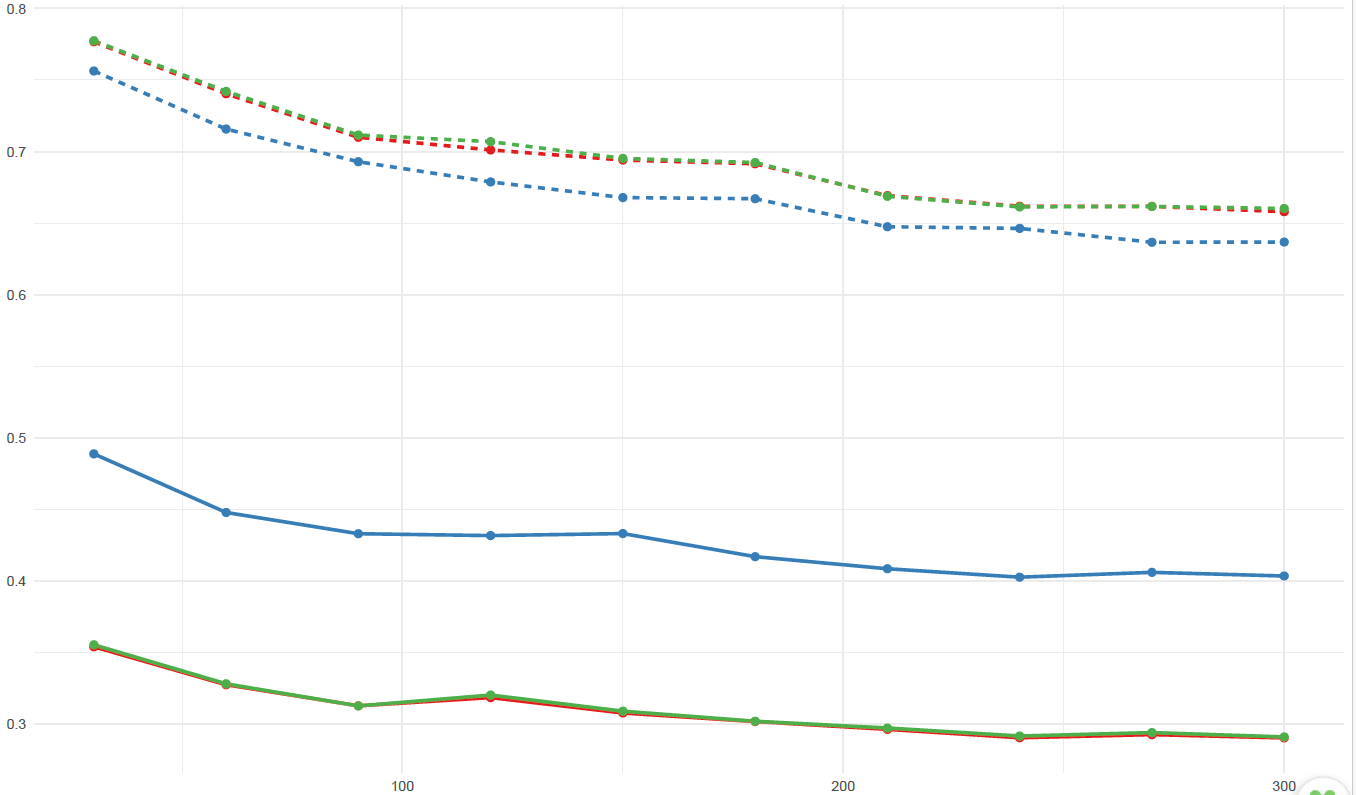
\includegraphics[width=0.75\linewidth]{Learning_curve.png}
    \caption{Aitchison distance as a function of training sample size for all three Random Forest models.}
    \label{fig:learning-curve}
  \end{figure}
}
\end{frame}


% ── IMPLEMENTATION ──────────────────────────────────────────
\begin{frame}{Implementation \& Code Access}

\vspace{1em}

\begin{itemize}[itemsep=1em]
  \item[\textcolor{blue}{\large$\blacktriangleright$}] Model developed in \textbf{Julia} for computational efficiency

  \item[\textcolor{blue}{\large$\blacktriangleright$}] Code available on \href{https://github.com/Xaleed/DirichletRandomForestJulia.git}{\textcolor{blue}{\textbf{GitHub}}}:

  \textcolor{blue}{\small https://github.com/Xaleed/DirichletRandomForestJulia.git}
  \begin{center}
    \qrcode{https://github.com/Xaleed/DirichletRandomForestJulia.git}
  \end{center}
\end{itemize}

\vspace{1.5em}

\end{frame}


% ── ALTERNATIVE TO MLE ──────────────────────────────────────
% FIX: removed duplicate \end{frame} that appeared here in original
\begin{frame}{Alternative to MLE}
\only<1>{
  \begin{block}{}
    One simple way to address this issue is to use the method of moments (MoM) as an alternative to maximum likelihood estimation (MLE). MoM gives an approximate solution but is much faster to compute.
  \end{block}
  \begin{block}{}
    We can also combine both approaches --- instead of using MoM in all nodes, we can selectively apply it only in nodes where we expect its results to be close to MLE. This helps reduce computation while still keeping good accuracy.
  \end{block}

  \resizebox{0.65\linewidth}{!}{%
  \begin{tabular}{|l|c|c|c|c|}
    \hline
    % FIX: was \multirow{Metric} — missing required arguments
    \multirow{2}{*}{Metric} & \multicolumn{2}{c|}{MLE} & \multicolumn{2}{c|}{MoM} \\
    \cline{2-5}
     & (Train) & (Test) & (Train) & (Test) \\
    \hline
    Aitchison Distance & 0.3901 & 0.7391 & 0.4068 & 0.7457 \\
    \hline
  \end{tabular}}
}
\end{frame}


% ── REAL DATA ───────────────────────────────────────────────
\begin{frame}{Data}

\begin{itemize}[label=\textbullet]
  \item We use soil texture data from Germany. The data comes from the 2018 LUCAS survey.

  \vspace{0.5em}

  \item We have around 1,785 observations. Each observation contains three components: clay, sand, and silt --- and together they always sum to one, which makes this compositional data.

  \vspace{0.5em}

  \item A total of \textbf{133 environmental covariates} (at $250 \times 250$ m resolution) were used as predictors, including climate, temperature, and vegetation-related variables.
\end{itemize}

\end{frame}


% ── SPATIAL DISTRIBUTION ────────────────────────────────────
\begin{frame}{Spatial Distribution of Soil Texture}

\begin{columns}
  \begin{column}{0.45\textwidth}
    \begin{itemize}
      \item[1.] Each point represents one \textbf{observation location} in Germany.
      \item[2.] The \textbf{colour} of each point indicates the value of the component: darker colours indicate \textbf{higher values}, lighter colours indicate \textbf{lower values}.
      \item[3.] \textbf{Clay:} higher values concentrated in the \textbf{south and centre}.
      \item[5.] \textbf{Sand:} higher values mostly in the \textbf{north and north-east}.
      \item[6.] \textbf{Silt:} more mixed pattern, with elevated values across the \textbf{central belt}.
    \end{itemize}
  \end{column}

  \begin{column}{0.55\textwidth}
    \only<1>{
      \begin{figure}
        \centering
        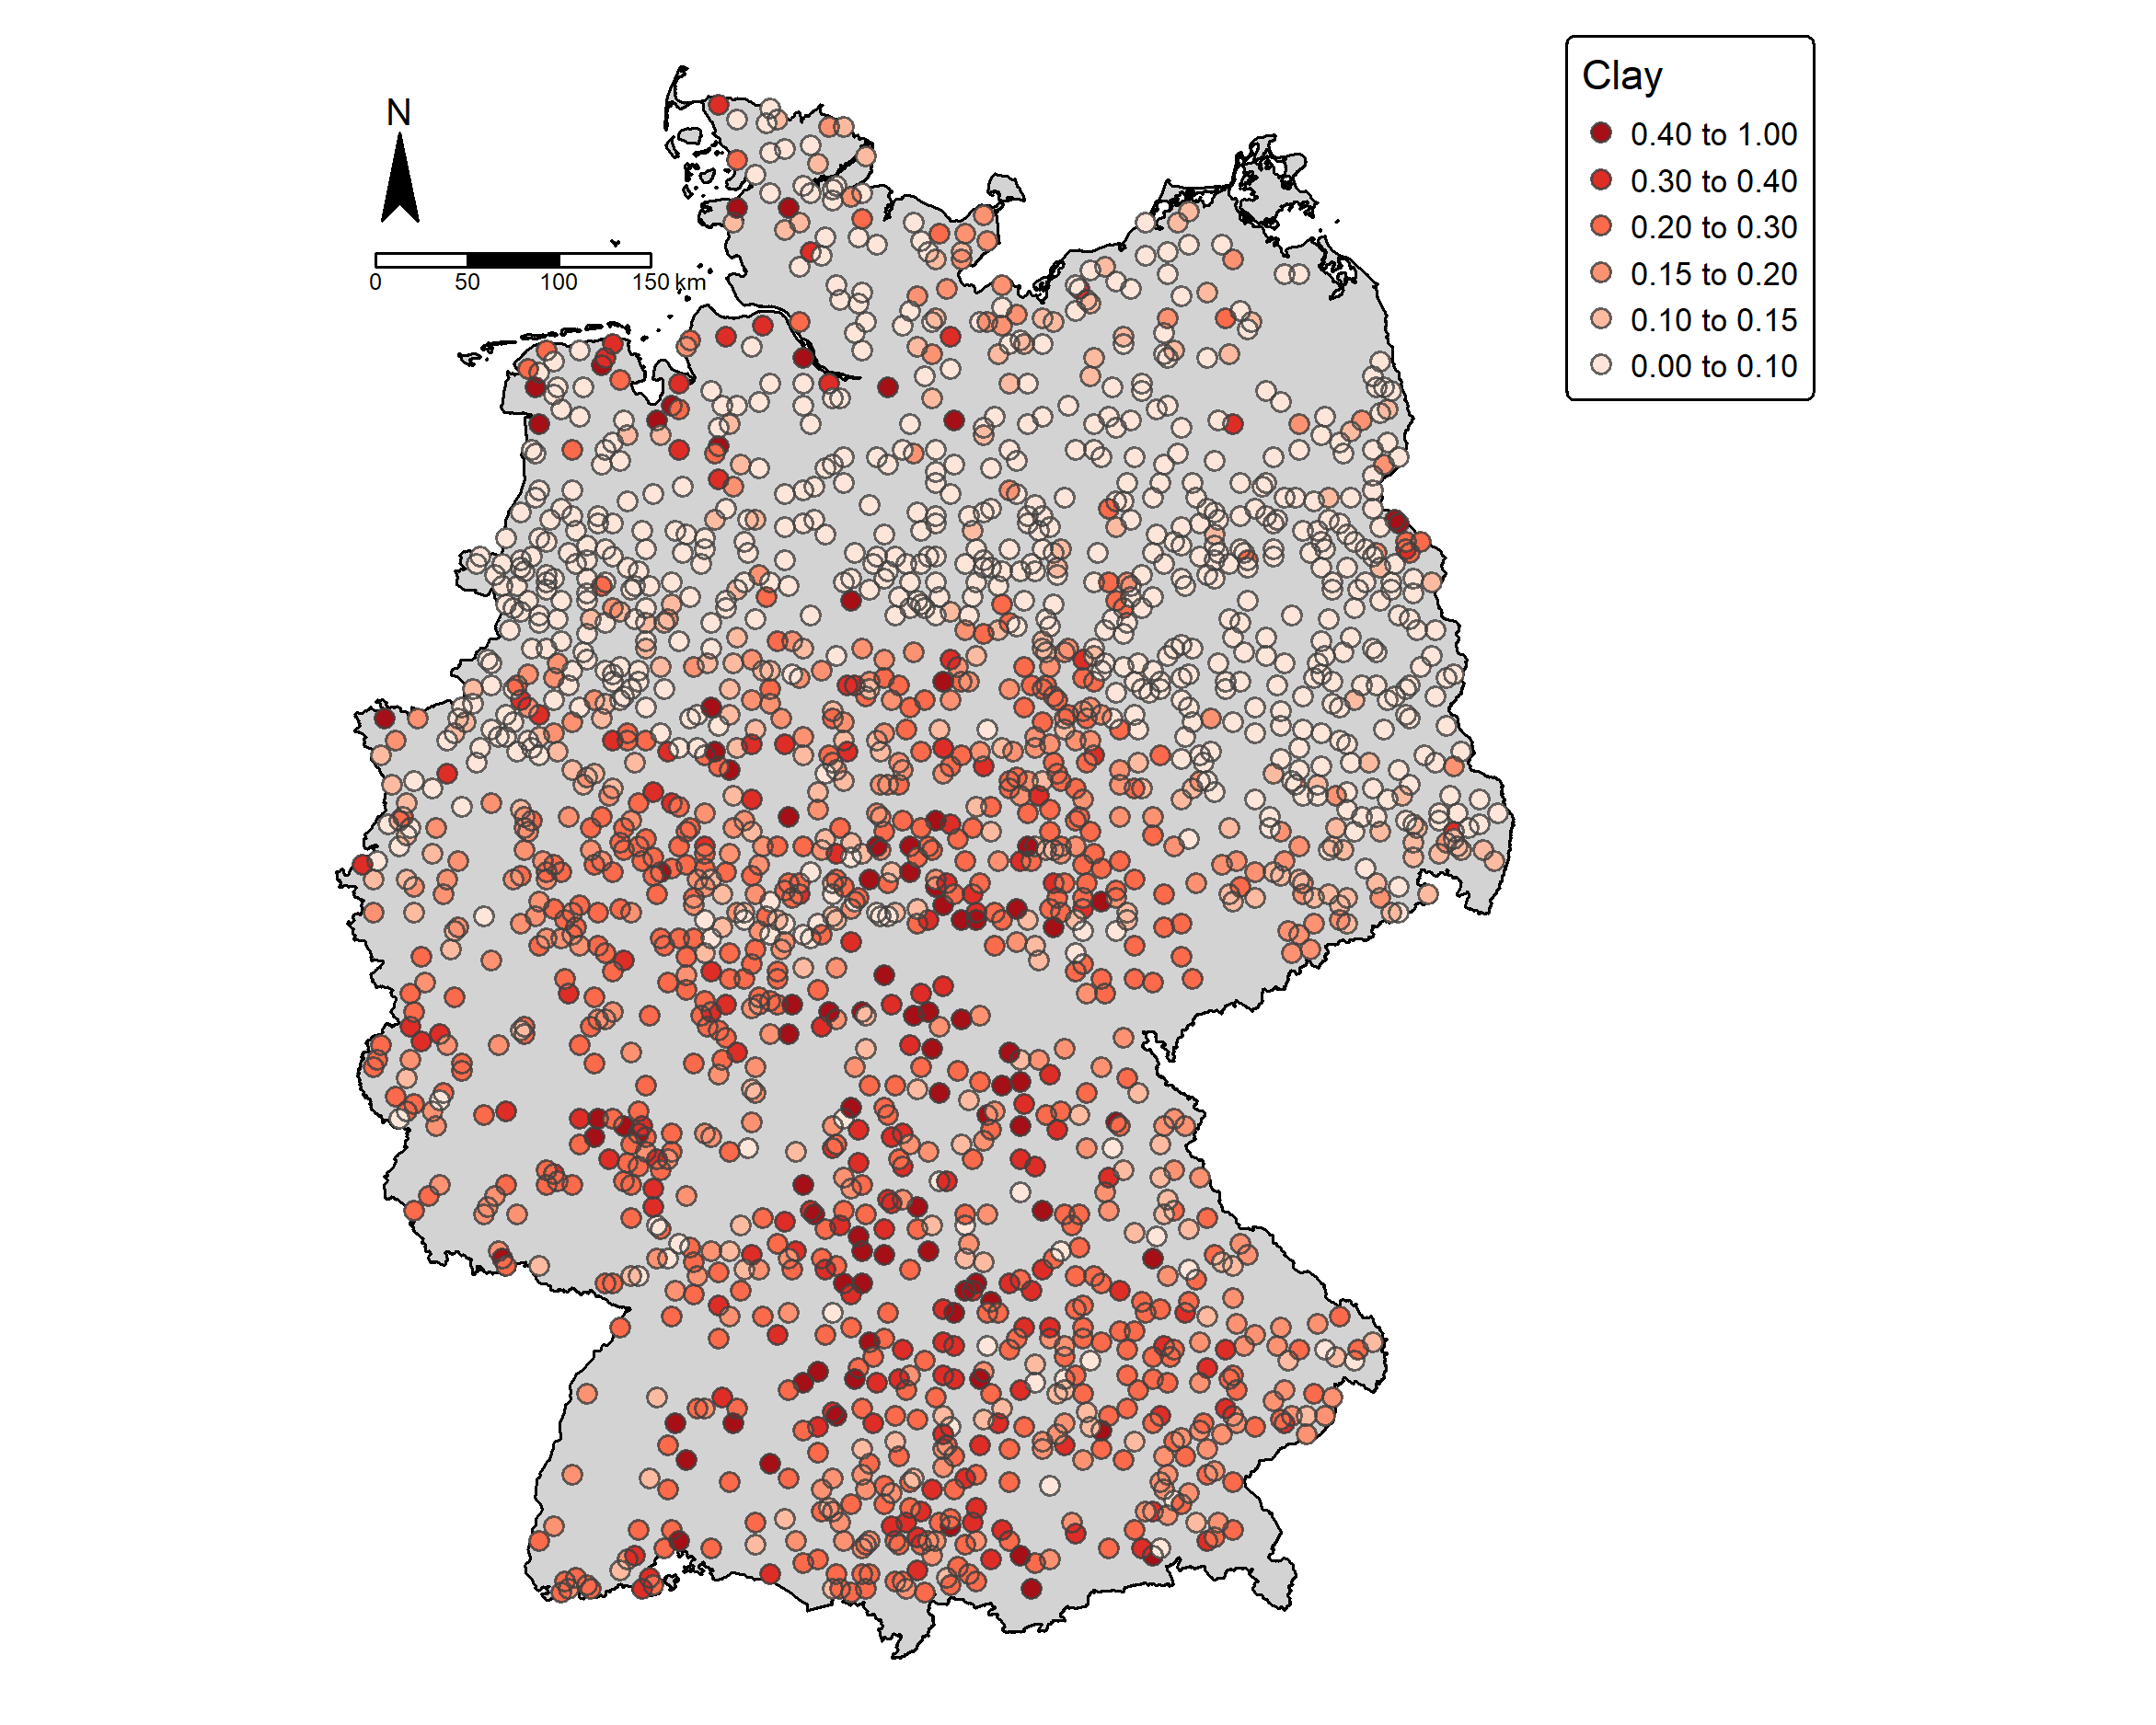
\includegraphics[width=\linewidth]{Figures/pointmap_clay.png}
        \caption{LUCAS soil texture observation locations in Germany: Clay.}
      \end{figure}
    }
    \only<2>{
      \begin{figure}
        \centering
        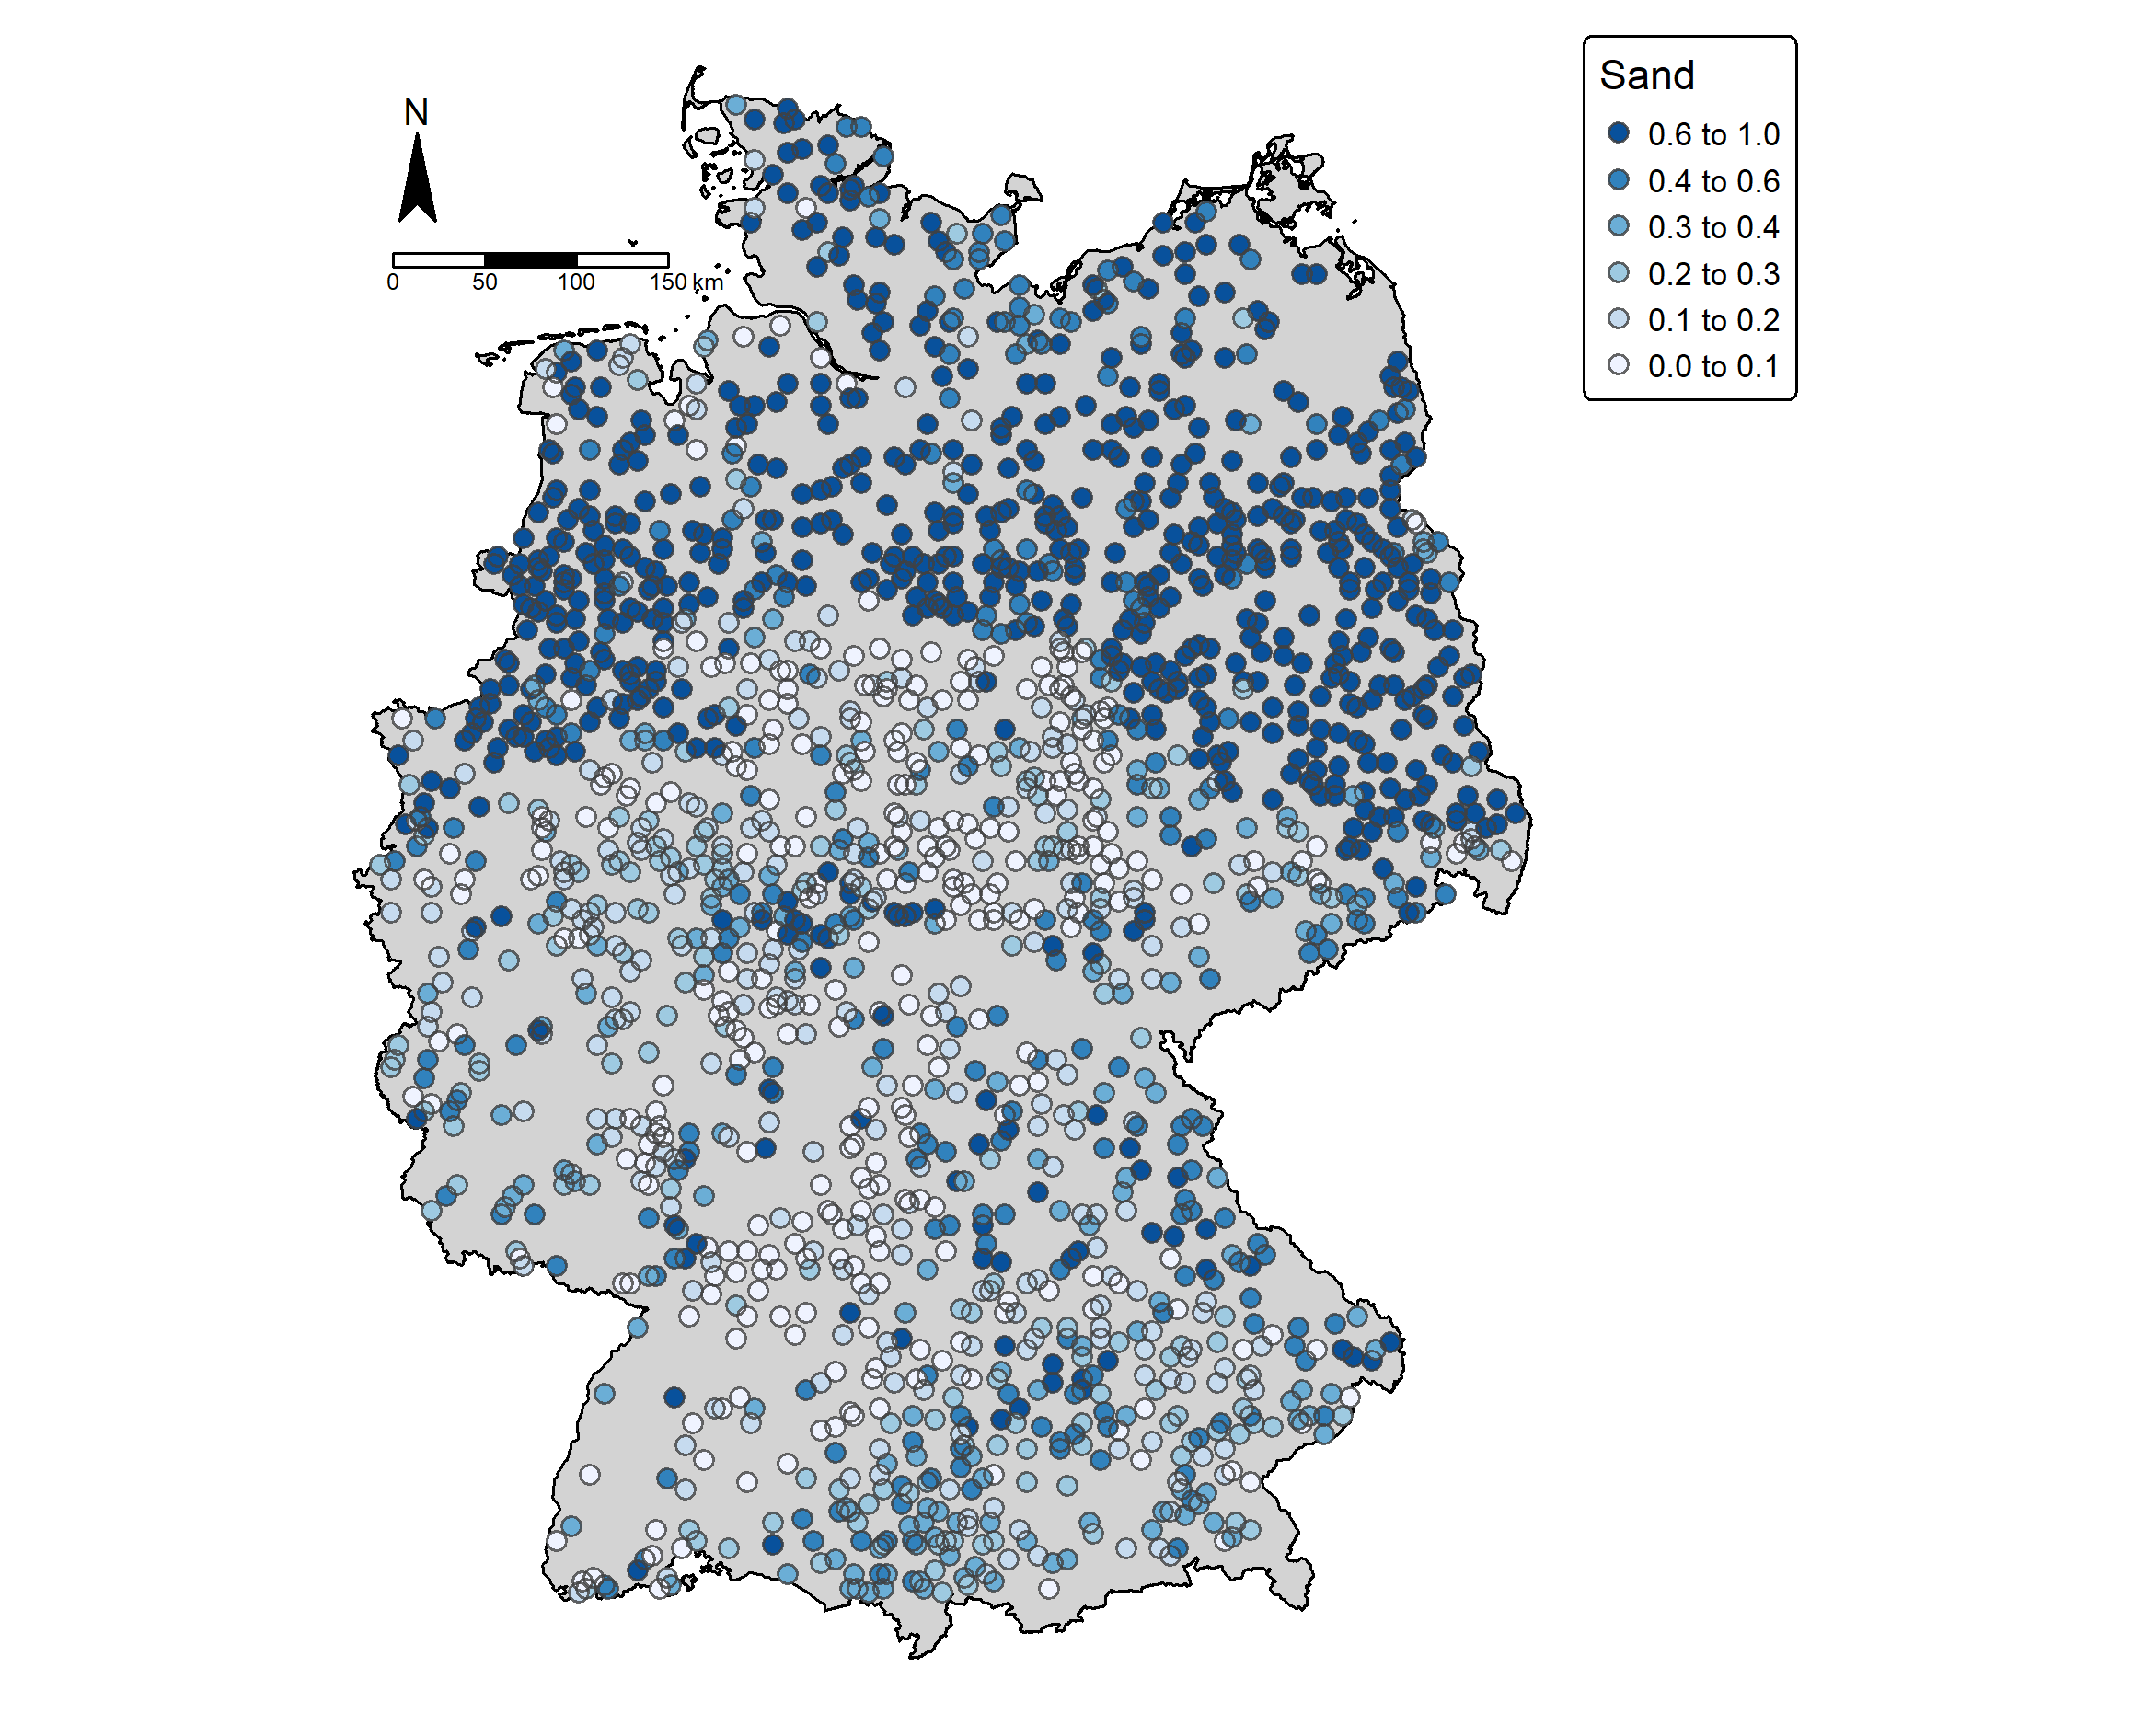
\includegraphics[width=\linewidth]{Figures/pointmap_sand.png}
        \caption{LUCAS soil texture observation locations in Germany: Sand.}
      \end{figure}
    }
    \only<3>{
      \begin{figure}
        \centering
        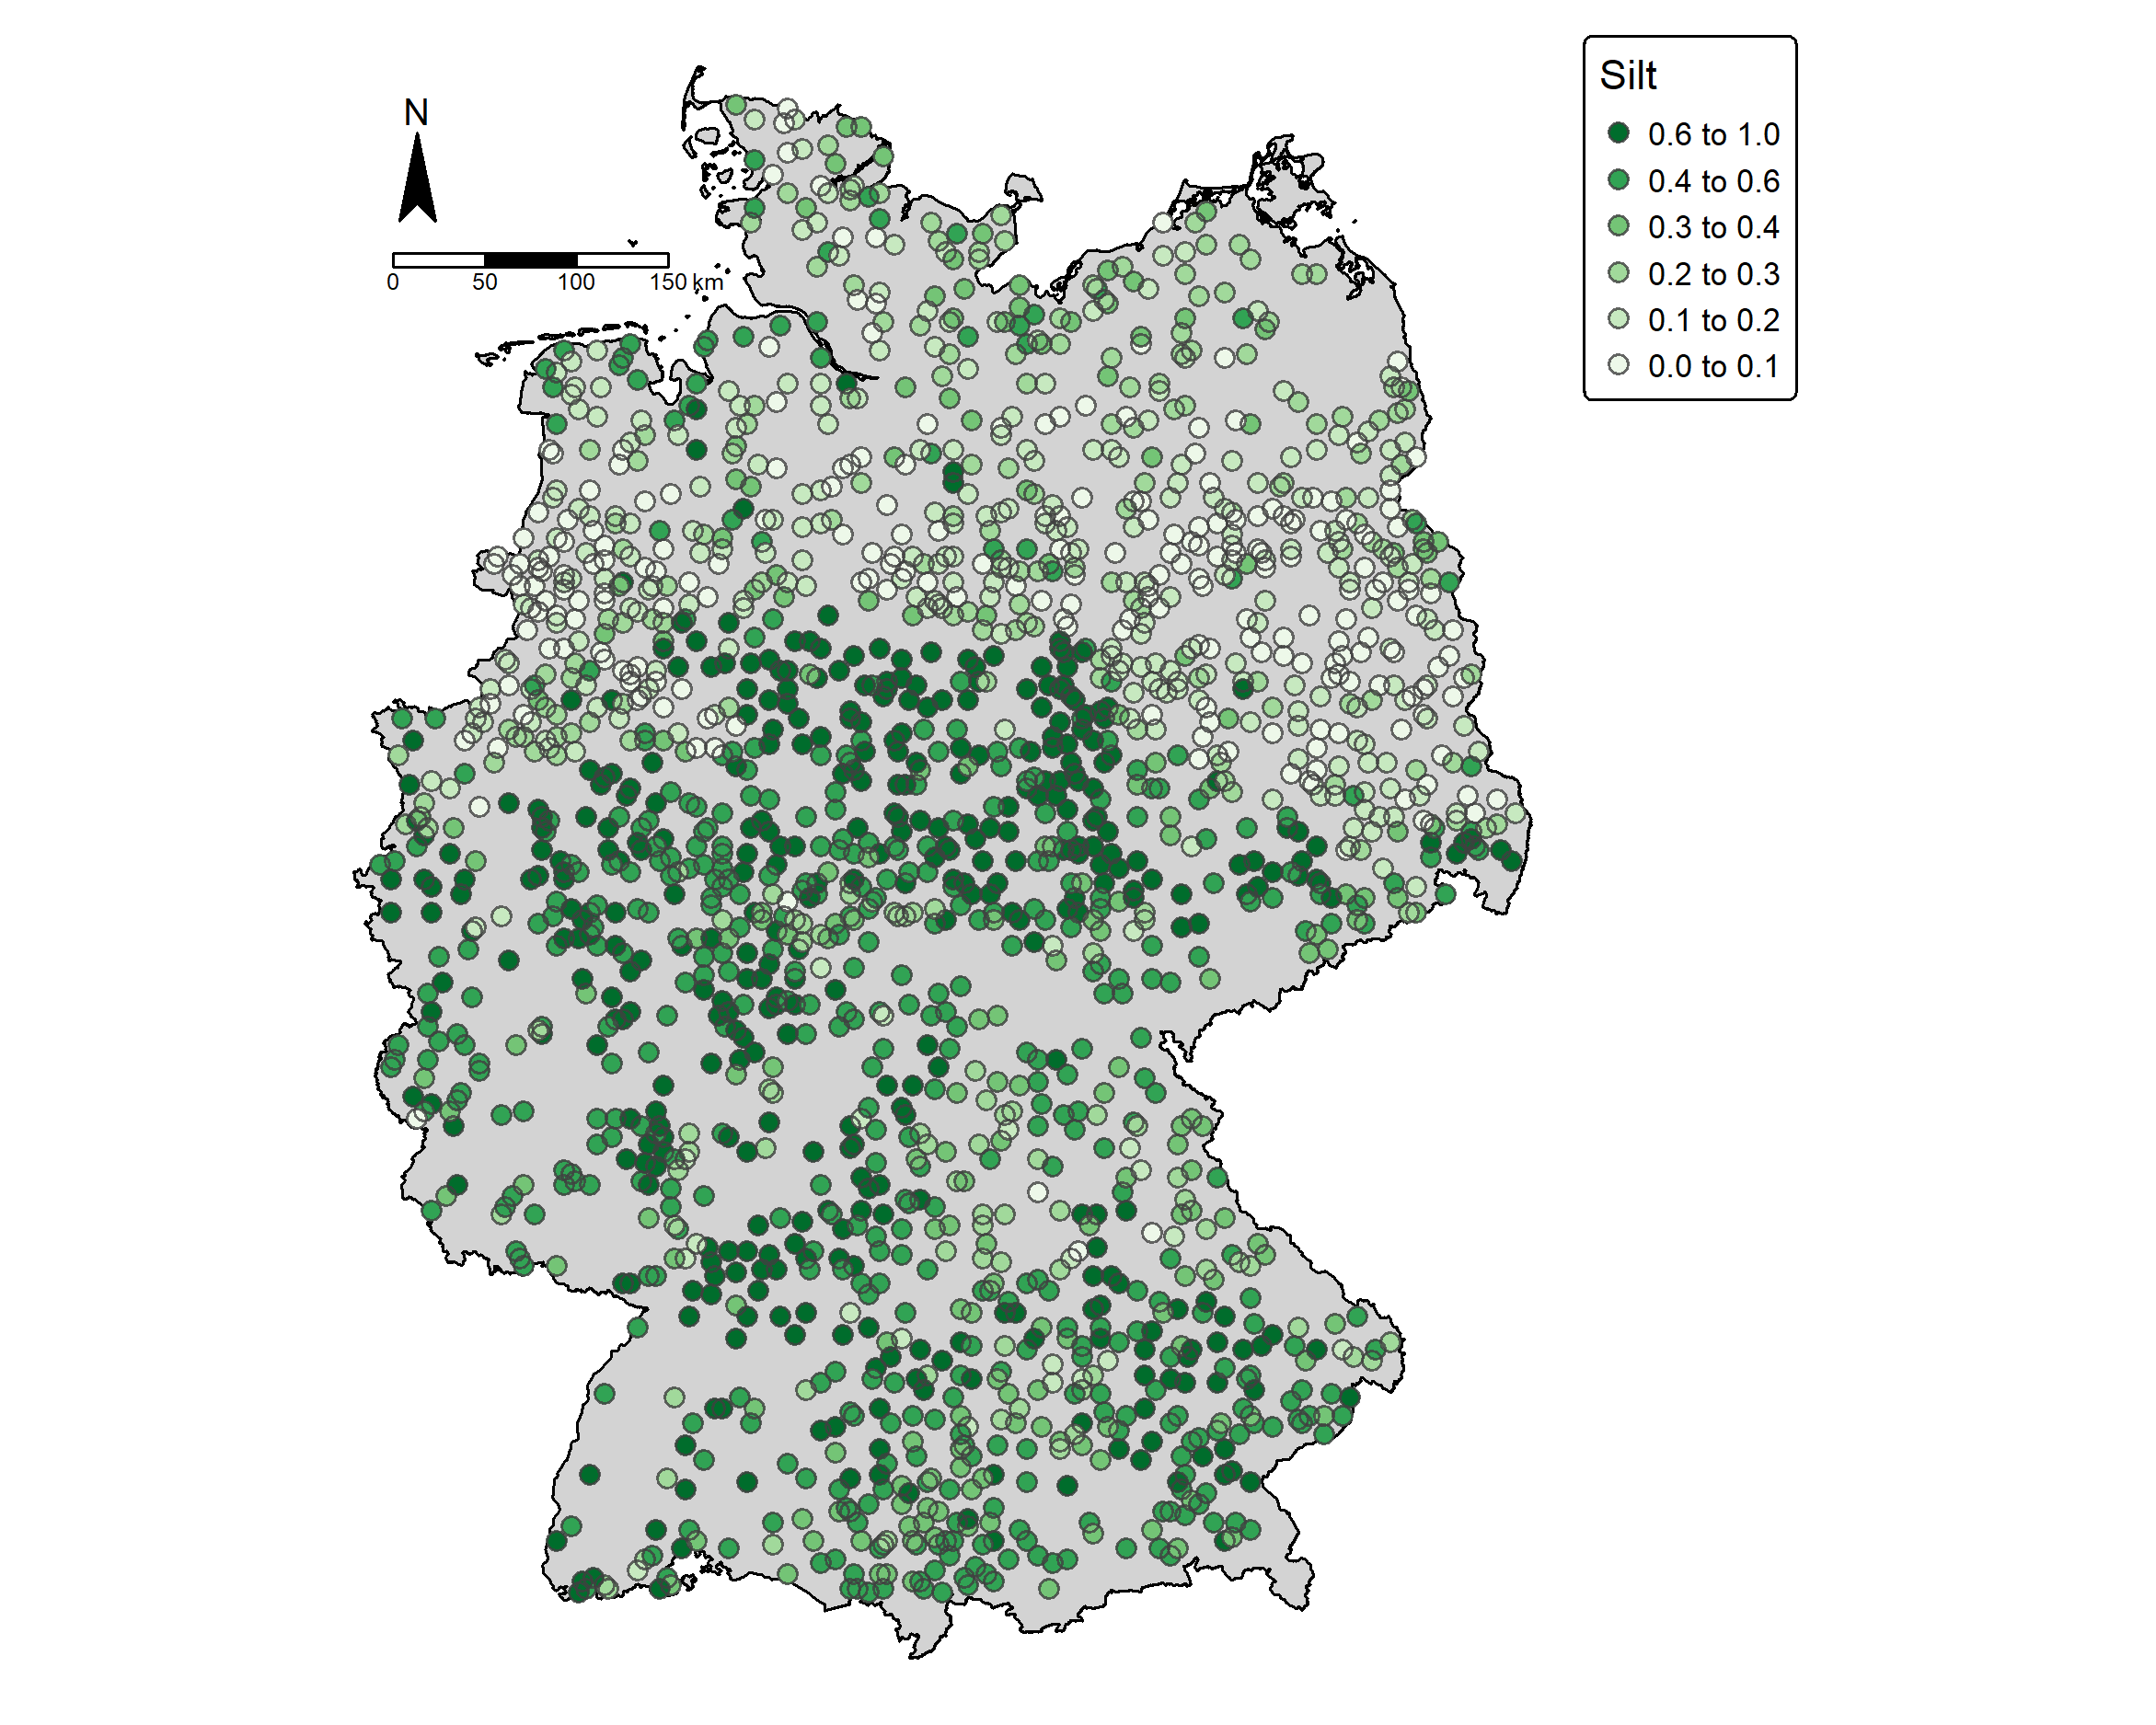
\includegraphics[width=\linewidth]{Figures/pointmap_silt.png}
        \caption{LUCAS soil texture observation locations in Germany: Silt.}
      \end{figure}
    }
  \end{column}
\end{columns}

\end{frame}


% ── TERNARY PLOT ────────────────────────────────────────────
\begin{frame}{Ternary Plot of Soil Texture}

\begin{columns}
  \begin{column}{0.45\textwidth}
    \begin{itemize}
      \item A \textbf{ternary plot} is a triangle where each corner represents $100\%$ of one component: clay, sand, or silt.
      \item Each \textbf{point} represents one observation, and its position shows the relative proportions of the three components.
      \item Points closer to a corner have a \textbf{higher proportion} of that component.
      \item Most observations cluster along the \textbf{sand--silt} edge, meaning few samples have high clay content.
      \item The spread of points reflects the \textbf{large variability} of sand and silt compared to clay.
    \end{itemize}
  \end{column}

  \begin{column}{0.55\textwidth}
    \begin{figure}
      \centering
      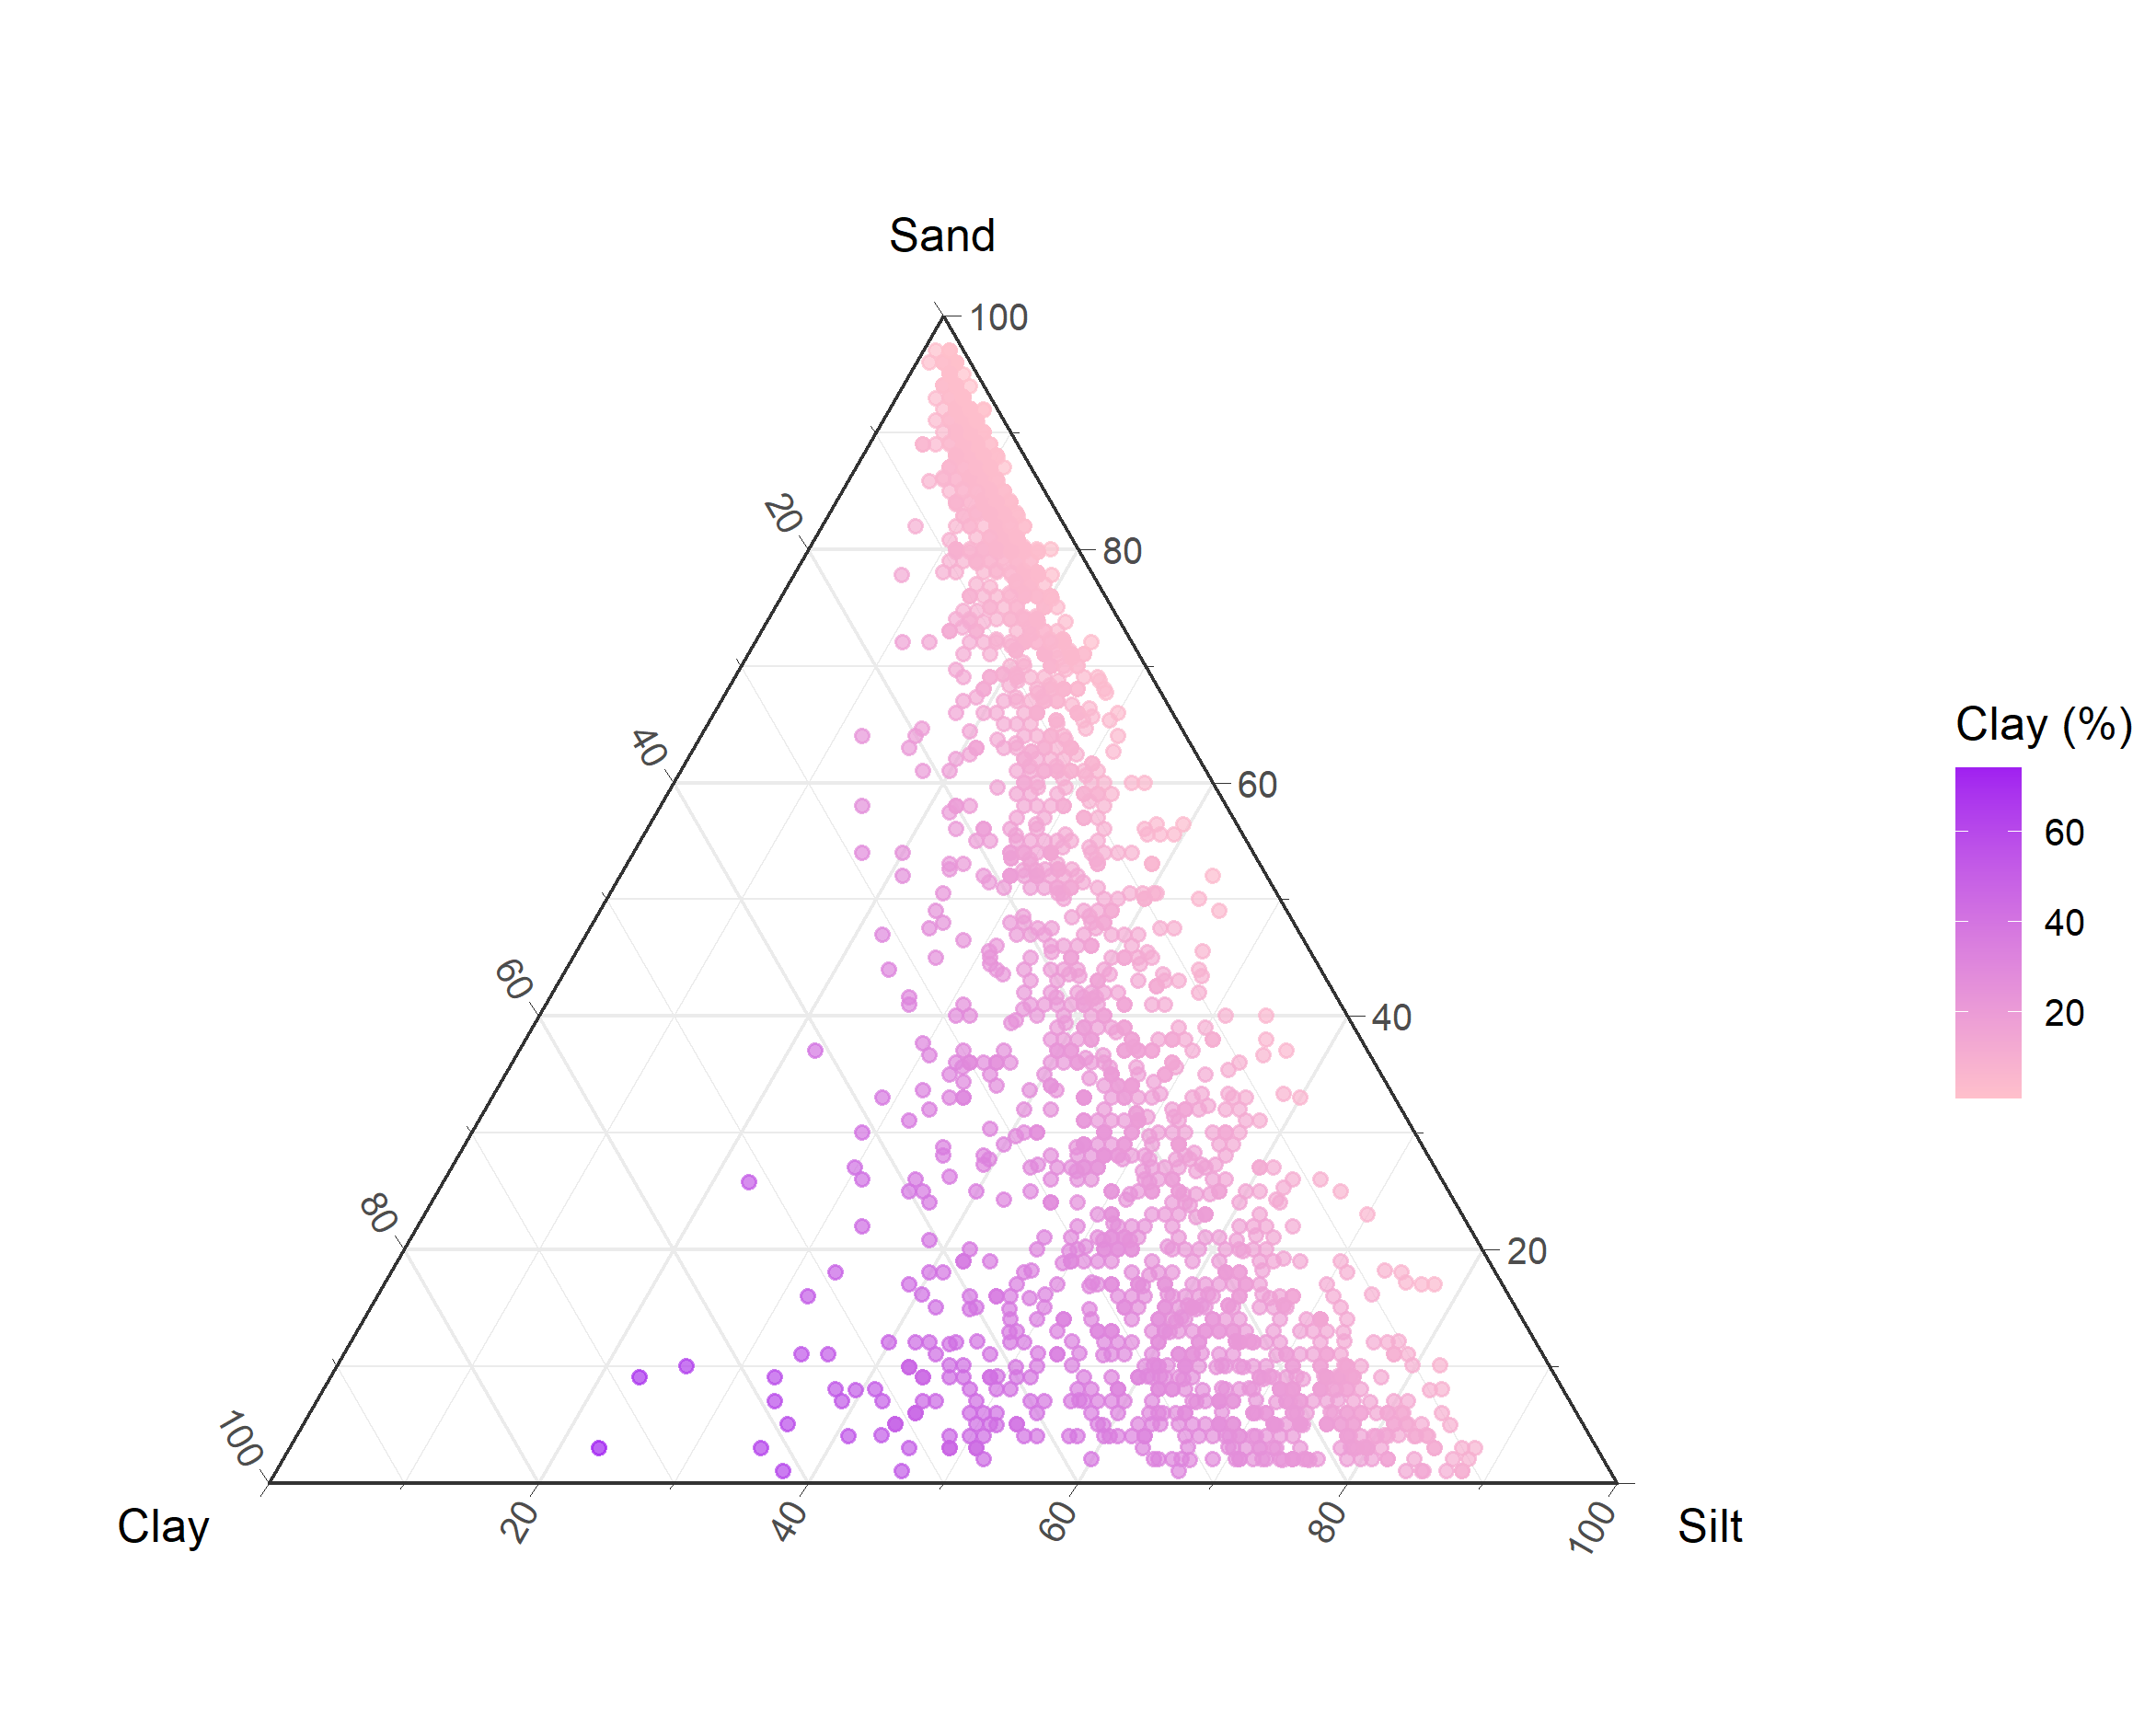
\includegraphics[width=\linewidth]{Figures/point_tern.png}
      \caption{Ternary plot of clay, sand, and silt distributions.}
    \end{figure}
  \end{column}
\end{columns}

\end{frame}


% ── MODELLING STRATEGIES ────────────────────────────────────
\begin{frame}{Modelling Strategies}

Five modelling approaches were compared:

\begin{table}
\centering\small
\begin{tabular}{lccc}
  \toprule
  Model & Joint estimation & Respects geometry & Transformation \\
  \midrule
  RF (raw)       & No  & No  & No  \\
  MRF (raw)      & Yes & No  & No  \\
  ilr-RF         & No  & Yes & Yes \\
  ilr-MRF        & Yes & Yes & Yes \\
  \textbf{DirRF} & Yes & Yes & No  \\
  \bottomrule
\end{tabular}
\caption{Summary of modelling strategies.}
\end{table}

\begin{itemize}
  \item RF and MRF on raw components serve as \textbf{baseline} approaches.
  \item \textbf{DirRF} works directly on the simplex without requiring any log-ratio transformation.
\end{itemize}

\end{frame}


% ── PARAMETER TUNING ────────────────────────────────────────
\begin{frame}{Parameter Tuning and Cross-Validation}

\begin{itemize}[label=\textbullet]
  \item All models were calibrated and evaluated using \textbf{10-fold nested cross-validation}.
  \vspace{0.5em}
  \item The same data folds were used for every model to ensure a \textbf{fair comparison} across methods.
  \vspace{0.5em}
  \item All random forest models were fitted with \textbf{500 trees}.
  \vspace{0.5em}
  \item Hyper-parameters were tuned by grid search:
    \begin{itemize}[label=\textbullet]
      \item minimum node size: $\{2, 5, 10\}$
      \item $m_{\mathrm{try}}$: $\{23, 29, 35, 41, 47, 53, 59, 65\}$
    \end{itemize}
  \vspace{0.5em}
  \item For DirRF, the minimum node size was fixed at $5$ for computational efficiency.
  \vspace{0.5em}
  \item Model performance was evaluated using:
    \begin{itemize}[label=\textbullet]
      \item Root Mean Squared Error (RMSE)
      \item Aitchison distance
    \end{itemize}
  \vspace{0.5em}
  \item For spatial comparison, models were refitted on the full data set using the best hyper-parameters selected from the inner folds.
\end{itemize}

\end{frame}


% ── RESULTS ─────────────────────────────────────────────────
\begin{frame}{Results: RMSE and Aitchison Distance}

\begin{table}
\centering\small
\caption{RMSE and Aitchison Distance (AID) across modelling approaches.}
\begin{tabular}{lccccc}
  \toprule
   & RF & ilr-RF & MRF & ilr-MRF & \textbf{DirRF} \\
  \midrule
  \multicolumn{6}{c}{\textbf{RMSE}} \\
  \midrule
  Clay       & 0.086 & 0.086 & 0.088 & 0.087 & \textbf{0.085} \\
  Sand       & 0.186 & 0.181 & 0.188 & 0.182 & \textbf{0.168} \\
  Silt       & 0.148 & 0.145 & 0.150 & 0.146 & \textbf{0.135} \\
  Aggregated & 0.140 & 0.137 & 0.142 & 0.138 & \textbf{0.130} \\
  \midrule
  \multicolumn{6}{c}{\textbf{Aitchison Distance (AID)}} \\
  \midrule
  AID & 0.852 & 0.788 & 0.861 & 0.798 & \textbf{0.766} \\
  \bottomrule
\end{tabular}
\end{table}

\begin{itemize}
  \item \textbf{DirRF} achieves the lowest RMSE across all components and the smallest AID.
  \item The largest gains are observed for \textbf{sand} and \textbf{silt}.
  \item ilr-based models only marginally outperform their untransformed counterparts.
\end{itemize}

\end{frame}